\documentclass[a4paper]{book}
\usepackage{a4wide}
\usepackage{makeidx}
\usepackage{graphicx}
\usepackage{multicol}
\usepackage{float}
\usepackage{listings}
\usepackage{color}
\usepackage{textcomp}
\usepackage{alltt}
\usepackage{times}
\usepackage{ifpdf}
\ifpdf
\usepackage[pdftex,
            pagebackref=true,
            colorlinks=true,
            linkcolor=blue,
            unicode
           ]{hyperref}
\else
\usepackage[ps2pdf,
            pagebackref=true,
            colorlinks=true,
            linkcolor=blue,
            unicode
           ]{hyperref}
\usepackage{pspicture}
\fi
\usepackage[utf8]{inputenc}
\usepackage{doxygen}
\lstset{language=C++,inputencoding=utf8,basicstyle=\footnotesize,breaklines=true,breakatwhitespace=true,tabsize=8,numbers=left }
\makeindex
\setcounter{tocdepth}{3}
\renewcommand{\footrulewidth}{0.4pt}
\begin{document}
\hypersetup{pageanchor=false}
\begin{titlepage}
\vspace*{7cm}
\begin{center}
{\Large Qcorr: A Digital Image Correlation Program implemented in QT4 \\[1ex]\large 1.0 }\\
\vspace*{1cm}
{\large Generated by Doxygen 1.6.1}\\
\vspace*{0.5cm}
{\small Sun Dec 6 21:50:54 2009}\\
\end{center}
\end{titlepage}
\clearemptydoublepage
\pagenumbering{roman}
\tableofcontents
\clearemptydoublepage
\pagenumbering{arabic}
\hypersetup{pageanchor=true}
\chapter{Todo List}
\label{todo}
\hypertarget{todo}{}
\label{todo__todo000001}
\hypertarget{todo__todo000001}{}
 \begin{description}
\item[Class \hyperlink{classQcorr}{Qcorr} ]\begin{itemize}
\item Add Stereo functionality to obtain disparity maps\end{itemize}


\end{description}

\chapter{Bug List}
\label{bug}
\hypertarget{bug}{}
\label{bug__bug000001}
\hypertarget{bug__bug000001}{}
 
\begin{DoxyDescription}
\item[Class \hyperlink{classQcorr}{Qcorr} ]
\begin{DoxyItemize}
\item Perhaps a few, but not noticed so far.
\end{DoxyItemize}


\end{DoxyDescription}
\chapter{Module Index}
\section{Modules}
Here is a list of all modules:\begin{DoxyCompactList}
\item \contentsline{section}{Qcorr}{\pageref{group__qcorr__mainwindow}}{}
\end{DoxyCompactList}

\chapter{Class Index}
\section{Class Hierarchy}
This inheritance list is sorted roughly, but not completely, alphabetically:\begin{CompactList}
\item \contentsline{section}{ImgLabel}{\pageref{classImgLabel}}{}
\item Ui\_\-QcorrClass\begin{CompactList}
\item Ui::QcorrClass\begin{CompactList}
\item \contentsline{section}{Qcorr}{\pageref{classQcorr}}{}
\end{CompactList}
\end{CompactList}
\end{CompactList}

\chapter{Class Index}
\section{Class List}
Here are the classes, structs, unions and interfaces with brief descriptions:\begin{CompactList}
\item\contentsline{section}{\hyperlink{classControlsWindow}{ControlsWindow} (Allows to modify parameters for the correlation operations, such as template size and scan interval. This class is a friend of \hyperlink{classQcorr}{Qcorr} )}{\pageref{classControlsWindow}}{}
\item\contentsline{section}{\hyperlink{classCorrMethod}{CorrMethod} (Dialog to select a method in which the correlation \char`\"{}template matching\char`\"{} operation will be based upon. The available correlation methods are the following:\begin{itemize}
\item CROSS\_\-CORR (cross correlation): \[ C(u,v) = \frac {\sum{\left\{T(x,y) * I(x-u,y-v)\right\}}} {\sqrt{ \sum{I(x-u,y-v)^2}}} \]\item SUM\_\-SQ\_\-DIFF (sum of squared differences): \[ C(u,v) = \frac {\sum{\left\{T(x,y)-I(x-u,y-v)\right\}^2}} {\sqrt{\sum{I(x-u,y-v)^2}}} \]\item CORR\_\-COEFF (correlation coefficient): \[ C(u,v) = \frac {\sum{\left\{(T(x,y)-T_{avg}) * (I(x-u,y-v)-I_{avg})\right\}}} {\sqrt{\sum{(T(x,y)-T_{avg})^2} * \sum{(I(x-u,y-v)-I_{avg})^2}}} \] \end{itemize}
)}{\pageref{classCorrMethod}}{}
\item\contentsline{section}{\hyperlink{classImgLabel}{ImgLabel} (A sub-classed label widget implemented with the purpose of displaying the reference image on the left panel )}{\pageref{classImgLabel}}{}
\item\contentsline{section}{\hyperlink{classQcorr}{Qcorr} (A Digital Image Correlation Program (Template Matcher and Pixel Disparity Mapping) implemented in QT4 )}{\pageref{classQcorr}}{}
\item\contentsline{section}{\hyperlink{classTargetImgLabel}{TargetImgLabel} (A sub-classed label widget implemented with the purpose of displaying the target image on the right panel )}{\pageref{classTargetImgLabel}}{}
\end{CompactList}

\chapter{Module Documentation}
\hypertarget{group__qcorr__mainwindow}{
\section{Qcorr}
\label{group__qcorr__mainwindow}\index{Qcorr@{Qcorr}}
}
\subsection*{Classes}
\begin{CompactItemize}
\item 
class \hyperlink{classQcorr}{Qcorr}
\begin{CompactList}\small\item\em A Digital Image Correlation Program (Template Matching and Pixel Disparity Finder) implemented in QT4. \item\end{CompactList}\end{CompactItemize}

\chapter{Class Documentation}
\input{classControlsWindow}
\include{classControlsWindow}
\include{classUi_1_1ControlsWindowClass}
\hypertarget{classCorrMethod}{
\section{CorrMethod Class Reference}
\label{classCorrMethod}\index{CorrMethod@{CorrMethod}}
}
Dialog to select a method in which the correlation \char`\"{}template matching\char`\"{} operation will be based upon. The available correlation methods are the following:\begin{itemize}
\item CROSS\_\-CORR (cross correlation): \[ C(u,v) = \frac {\sum{\left\{T(x,y) * I(x-u,y-v)\right\}}} {\sqrt{ \sum{I(x-u,y-v)^2}}} \]\item SUM\_\-SQ\_\-DIFF (sum of squared differences): \[ C(u,v) = \frac {\sum{\left\{T(x,y)-I(x-u,y-v)\right\}^2}} {\sqrt{\sum{I(x-u,y-v)^2}}} \]\item CORR\_\-COEFF (correlation coefficient): \[ C(u,v) = \frac {\sum{\left\{(T(x,y)-T_{avg}) * (I(x-u,y-v)-I_{avg})\right\}}} {\sqrt{\sum{(T(x,y)-T_{avg})^2} * \sum{(I(x-u,y-v)-I_{avg})^2}}} \]. \end{itemize}
 


{\tt \#include $<$src/corrmethod.h$>$}

\subsection*{Public Member Functions}
\begin{CompactItemize}
\item 
\hypertarget{classCorrMethod_bdc14398267291249d40158e133cf68b}{
\hyperlink{classCorrMethod_bdc14398267291249d40158e133cf68b}{CorrMethod} (QWidget $\ast$parent=0)}
\label{classCorrMethod_bdc14398267291249d40158e133cf68b}

\begin{CompactList}\small\item\em Constructor for the \hyperlink{classCorrMethod}{CorrMethod} class. \item\end{CompactList}\item 
int \hyperlink{classCorrMethod_3eeafdd901560c1fa92be75d4ed58872}{getMethod} ()
\begin{CompactList}\small\item\em Retrieve the selected method to be used in the correlation process. \item\end{CompactList}\end{CompactItemize}
\subsection*{Private Slots}
\begin{CompactItemize}
\item 
\hypertarget{classCorrMethod_87e628d7ef6facc9a402880d7e01ea36}{
void \hyperlink{classCorrMethod_87e628d7ef6facc9a402880d7e01ea36}{cancelMethod} ()}
\label{classCorrMethod_87e628d7ef6facc9a402880d7e01ea36}

\begin{CompactList}\small\item\em Q\_\-SLOT to cancel the method selection dialog. \item\end{CompactList}\item 
\hypertarget{classCorrMethod_7522197ac15c7563aee8d15d0cff3d95}{
void \hyperlink{classCorrMethod_7522197ac15c7563aee8d15d0cff3d95}{chooseMethod} ()}
\label{classCorrMethod_7522197ac15c7563aee8d15d0cff3d95}

\begin{CompactList}\small\item\em Q\_\-SLOT to store the method selection from the dialog. \item\end{CompactList}\end{CompactItemize}
\subsection*{Private Attributes}
\begin{CompactItemize}
\item 
int \hyperlink{classCorrMethod_3e64e1a2c9eabff57b7e58eaff13f45f}{m\_\-nChosenMethod}
\item 
\hypertarget{classCorrMethod_866bb1b72235d777ca96a6ce9701f9f6}{
Ui::CorrMethodClass \hyperlink{classCorrMethod_866bb1b72235d777ca96a6ce9701f9f6}{ui}}
\label{classCorrMethod_866bb1b72235d777ca96a6ce9701f9f6}

\begin{CompactList}\small\item\em The Qt GUI form for this class, so its widgets can be accessed and manipulated. \item\end{CompactList}\end{CompactItemize}


\subsection{Detailed Description}
Dialog to select a method in which the correlation \char`\"{}template matching\char`\"{} operation will be based upon. The available correlation methods are the following:\begin{itemize}
\item CROSS\_\-CORR (cross correlation): \[ C(u,v) = \frac {\sum{\left\{T(x,y) * I(x-u,y-v)\right\}}} {\sqrt{ \sum{I(x-u,y-v)^2}}} \]\item SUM\_\-SQ\_\-DIFF (sum of squared differences): \[ C(u,v) = \frac {\sum{\left\{T(x,y)-I(x-u,y-v)\right\}^2}} {\sqrt{\sum{I(x-u,y-v)^2}}} \]\item CORR\_\-COEFF (correlation coefficient): \[ C(u,v) = \frac {\sum{\left\{(T(x,y)-T_{avg}) * (I(x-u,y-v)-I_{avg})\right\}}} {\sqrt{\sum{(T(x,y)-T_{avg})^2} * \sum{(I(x-u,y-v)-I_{avg})^2}}} \]. \end{itemize}


Definition at line 30 of file corrmethod.h.

\subsection{Member Function Documentation}
\hypertarget{classCorrMethod_3eeafdd901560c1fa92be75d4ed58872}{
\index{CorrMethod@{CorrMethod}!getMethod@{getMethod}}
\index{getMethod@{getMethod}!CorrMethod@{CorrMethod}}
\subsubsection[{getMethod}]{\setlength{\rightskip}{0pt plus 5cm}int CorrMethod::getMethod ()}}
\label{classCorrMethod_3eeafdd901560c1fa92be75d4ed58872}


Retrieve the selected method to be used in the correlation process. 

Returns the selected method in which the correlation \char`\"{}template matching\char`\"{} operation will be based upon. From the global enumeration MethodOfCorrelation, the available correlation methods are: N0\_\-CORR\_\-METHOD = 0, CROSS\_\-CORR = 1, SUM\_\-SQ\_\-DIFF = 2, or CORR\_\-COEFF = 3

\begin{Desc}
\item[Returns:]selected correlation method (from global enumeration MethodOfCorrelation defined in \hyperlink{globals_8h-source}{globals.h}). The available correlation methods are: N0\_\-CORR\_\-METHOD = 0, CROSS\_\-CORR = 1, SUM\_\-SQ\_\-DIFF = 2, or CORR\_\-COEFF = 3 \end{Desc}


Definition at line 22 of file corrmethod.cpp.

References m\_\-nChosenMethod.

Referenced by Qcorr::correlate().

\subsection{Member Data Documentation}
\hypertarget{classCorrMethod_3e64e1a2c9eabff57b7e58eaff13f45f}{
\index{CorrMethod@{CorrMethod}!m\_\-nChosenMethod@{m\_\-nChosenMethod}}
\index{m\_\-nChosenMethod@{m\_\-nChosenMethod}!CorrMethod@{CorrMethod}}
\subsubsection[{m\_\-nChosenMethod}]{\setlength{\rightskip}{0pt plus 5cm}int {\bf CorrMethod::m\_\-nChosenMethod}\hspace{0.3cm}{\tt  \mbox{[}private\mbox{]}}}}
\label{classCorrMethod_3e64e1a2c9eabff57b7e58eaff13f45f}


The selected method in which the correlation \char`\"{}template matching\char`\"{} operation will be based upon. From the global enumeration MethodOfCorrelation, the available correlation methods are: N0\_\-CORR\_\-METHOD = 0, CROSS\_\-CORR = 1, SUM\_\-SQ\_\-DIFF = 2, or CORR\_\-COEFF = 3 

Definition at line 61 of file corrmethod.h.

Referenced by cancelMethod(), chooseMethod(), CorrMethod(), and getMethod().

The documentation for this class was generated from the following files:\begin{CompactItemize}
\item 
src/corrmethod.h\item 
src/corrmethod.cpp\end{CompactItemize}

\hypertarget{classUi_1_1CorrMethodClass}{
\section{Ui::CorrMethodClass Class Reference}
\label{classUi_1_1CorrMethodClass}\index{Ui::CorrMethodClass@{Ui::CorrMethodClass}}
}
Inheritance diagram for Ui::CorrMethodClass::\begin{figure}[H]
\begin{center}
\leavevmode
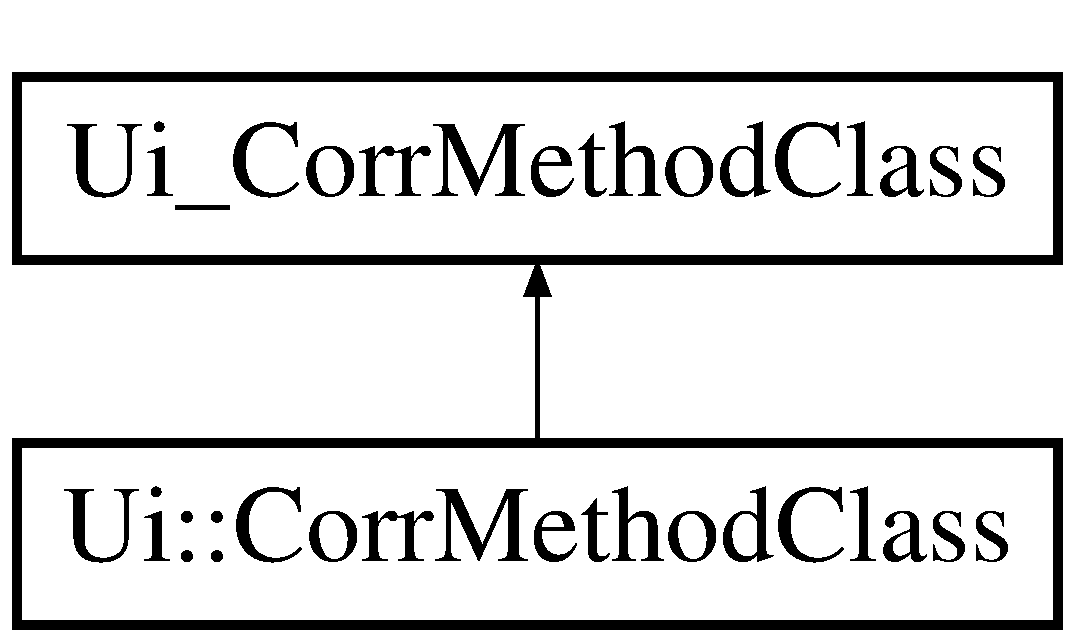
\includegraphics[height=2cm]{classUi_1_1CorrMethodClass}
\end{center}
\end{figure}


\subsection{Detailed Description}


Definition at line 132 of file ui\_\-corrmethod.h.

The documentation for this class was generated from the following file:\begin{DoxyCompactItemize}
\item 
ui\_\-corrmethod.h\end{DoxyCompactItemize}

\hypertarget{classImgLabel}{
\section{ImgLabel Class Reference}
\label{classImgLabel}\index{ImgLabel@{ImgLabel}}
}
\subsection*{Public Member Functions}
\begin{DoxyCompactItemize}
\item 
\hypertarget{classImgLabel_a69e37830ecfccbd824166d03fc9c248d}{
{\bfseries ImgLabel} (\hyperlink{classQcorr}{Qcorr} $\ast$parentWindow, QWidget $\ast$parent=0)}
\label{classImgLabel_a69e37830ecfccbd824166d03fc9c248d}

\end{DoxyCompactItemize}
\subsection*{Protected Member Functions}
\begin{DoxyCompactItemize}
\item 
\hypertarget{classImgLabel_a20d52d626aa1a1d6cebe3f7e2c33e295}{
void {\bfseries mousePressEvent} (QMouseEvent $\ast$event)}
\label{classImgLabel_a20d52d626aa1a1d6cebe3f7e2c33e295}

\item 
\hypertarget{classImgLabel_a935514f1ec077f7c817fb057a16d8c4d}{
void {\bfseries mouseMoveEvent} (QMouseEvent $\ast$event)}
\label{classImgLabel_a935514f1ec077f7c817fb057a16d8c4d}

\item 
\hypertarget{classImgLabel_accc9e0b19e5e7873a8493f0d7e03c65b}{
void {\bfseries mouseReleaseEvent} (QMouseEvent $\ast$event)}
\label{classImgLabel_accc9e0b19e5e7873a8493f0d7e03c65b}

\end{DoxyCompactItemize}
\subsection*{Private Member Functions}
\begin{DoxyCompactItemize}
\item 
\hypertarget{classImgLabel_a8a433cfccabf949ad3e975af3f09c120}{
void {\bfseries setTemplateFlags} (bool status)}
\label{classImgLabel_a8a433cfccabf949ad3e975af3f09c120}

\item 
\hypertarget{classImgLabel_aa71c0202c48be349b4fb0813891df43a}{
void {\bfseries checkTemplateRegions} (int mouseX, int mouseY)}
\label{classImgLabel_aa71c0202c48be349b4fb0813891df43a}

\item 
\hypertarget{classImgLabel_af8fb1abf00b305d1ba4d8b4745b59692}{
void {\bfseries displayCoordinatesOnStatusLabel} (QPoint \&point0, QPoint \&point1)}
\label{classImgLabel_af8fb1abf00b305d1ba4d8b4745b59692}

\end{DoxyCompactItemize}
\subsection*{Private Attributes}
\begin{DoxyCompactItemize}
\item 
\hypertarget{classImgLabel_abf77749e36bca018728bde2fc9a974eb}{
\hyperlink{classQcorr}{Qcorr} $\ast$ {\bfseries m\_\-parentWindow}}
\label{classImgLabel_abf77749e36bca018728bde2fc9a974eb}

\item 
\hypertarget{classImgLabel_aa62e5311b110d0551158c93c6c90e4cf}{
QRubberBand $\ast$ {\bfseries m\_\-rubberBand}}
\label{classImgLabel_aa62e5311b110d0551158c93c6c90e4cf}

\item 
\hypertarget{classImgLabel_afbbcbd660b7ef7c6048286ac5e350343}{
QPoint {\bfseries m\_\-originPoint}}
\label{classImgLabel_afbbcbd660b7ef7c6048286ac5e350343}

\item 
\hypertarget{classImgLabel_a6309ebb41fd14f64eb552e772c3bad25}{
QPoint {\bfseries m\_\-finalPoint}}
\label{classImgLabel_a6309ebb41fd14f64eb552e772c3bad25}

\item 
\hypertarget{classImgLabel_a24136f0f97b3f157721c07091a8261ac}{
QPoint {\bfseries m\_\-currentPressedPoint}}
\label{classImgLabel_a24136f0f97b3f157721c07091a8261ac}

\item 
\hypertarget{classImgLabel_a5818aa44b47111a75d4f1d4b749f6ba1}{
QPoint {\bfseries m\_\-labelUpperLeftCornerPoint}}
\label{classImgLabel_a5818aa44b47111a75d4f1d4b749f6ba1}

\item 
\hypertarget{classImgLabel_ae9c219000c7ccb81a73f9784ba9df23b}{
QPoint {\bfseries m\_\-labelLowerRightCornerPoint}}
\label{classImgLabel_ae9c219000c7ccb81a73f9784ba9df23b}

\item 
\hypertarget{classImgLabel_ad58eb83a86663876080a2e24ad016b39}{
QPoint {\bfseries m\_\-mousePosPoint1}}
\label{classImgLabel_ad58eb83a86663876080a2e24ad016b39}

\item 
\hypertarget{classImgLabel_a5d8c18646dda1aaf5c574ed88b63b0ee}{
QPoint {\bfseries m\_\-mousePosPoint2}}
\label{classImgLabel_a5d8c18646dda1aaf5c574ed88b63b0ee}

\item 
\hypertarget{classImgLabel_ab7550fba92f0346edd4a61c1a84eee4d}{
bool {\bfseries m\_\-bMouseIsPressed}}
\label{classImgLabel_ab7550fba92f0346edd4a61c1a84eee4d}

\item 
\hypertarget{classImgLabel_a45fe85b4d6b6da14b556c13284624145}{
bool {\bfseries m\_\-bStartedTemplateSelection}}
\label{classImgLabel_a45fe85b4d6b6da14b556c13284624145}

\item 
\hypertarget{classImgLabel_a990abf371f11243a65aa323bfad1cf10}{
bool {\bfseries m\_\-bMouseInTemplateRegion}}
\label{classImgLabel_a990abf371f11243a65aa323bfad1cf10}

\item 
\hypertarget{classImgLabel_ad4858784cd8aa7a53f948bb42ae7b996}{
bool {\bfseries m\_\-bMouseAtTemplateTopEdge}}
\label{classImgLabel_ad4858784cd8aa7a53f948bb42ae7b996}

\item 
\hypertarget{classImgLabel_a6d005e4bb487858c70d4d14564e4a095}{
bool {\bfseries m\_\-bMouseAtTemplateBottomEdge}}
\label{classImgLabel_a6d005e4bb487858c70d4d14564e4a095}

\item 
\hypertarget{classImgLabel_a921c1163775a86236d44d84e11172177}{
bool {\bfseries m\_\-bMouseAtTemplateLeftEdge}}
\label{classImgLabel_a921c1163775a86236d44d84e11172177}

\item 
\hypertarget{classImgLabel_afa3d9dc393d218e31b71f3e34bc79f9c}{
bool {\bfseries m\_\-bMouseAtTemplateRightEdge}}
\label{classImgLabel_afa3d9dc393d218e31b71f3e34bc79f9c}

\item 
\hypertarget{classImgLabel_a8440c20742b16b7b2bdceebe3e9f3302}{
int {\bfseries m\_\-nXNewPos}}
\label{classImgLabel_a8440c20742b16b7b2bdceebe3e9f3302}

\item 
\hypertarget{classImgLabel_a2060dad81295d4e6f87328108f97d15f}{
int {\bfseries m\_\-nYNewPos}}
\label{classImgLabel_a2060dad81295d4e6f87328108f97d15f}

\end{DoxyCompactItemize}
\subsection*{Friends}
\begin{DoxyCompactItemize}
\item 
\hypertarget{classImgLabel_ae86bc9b92f374c5f78097881af49364d}{
class \hyperlink{classImgLabel_ae86bc9b92f374c5f78097881af49364d}{Qcorr}}
\label{classImgLabel_ae86bc9b92f374c5f78097881af49364d}

\end{DoxyCompactItemize}


\subsection{Detailed Description}


Definition at line 19 of file imgLabel.h.

The documentation for this class was generated from the following files:\begin{DoxyCompactItemize}
\item 
src/imgLabel.h\item 
src/imgLabel.cpp\end{DoxyCompactItemize}

\hypertarget{classImgLabel}{
\section{ImgLabel Class Reference}
\label{classImgLabel}\index{ImgLabel@{ImgLabel}}
}
\subsection*{Public Member Functions}
\begin{DoxyCompactItemize}
\item 
\hypertarget{classImgLabel_a69e37830ecfccbd824166d03fc9c248d}{
{\bfseries ImgLabel} (\hyperlink{classQcorr}{Qcorr} $\ast$parentWindow, QWidget $\ast$parent=0)}
\label{classImgLabel_a69e37830ecfccbd824166d03fc9c248d}

\end{DoxyCompactItemize}
\subsection*{Protected Member Functions}
\begin{DoxyCompactItemize}
\item 
\hypertarget{classImgLabel_a20d52d626aa1a1d6cebe3f7e2c33e295}{
void {\bfseries mousePressEvent} (QMouseEvent $\ast$event)}
\label{classImgLabel_a20d52d626aa1a1d6cebe3f7e2c33e295}

\item 
\hypertarget{classImgLabel_a935514f1ec077f7c817fb057a16d8c4d}{
void {\bfseries mouseMoveEvent} (QMouseEvent $\ast$event)}
\label{classImgLabel_a935514f1ec077f7c817fb057a16d8c4d}

\item 
\hypertarget{classImgLabel_accc9e0b19e5e7873a8493f0d7e03c65b}{
void {\bfseries mouseReleaseEvent} (QMouseEvent $\ast$event)}
\label{classImgLabel_accc9e0b19e5e7873a8493f0d7e03c65b}

\end{DoxyCompactItemize}
\subsection*{Private Member Functions}
\begin{DoxyCompactItemize}
\item 
\hypertarget{classImgLabel_a8a433cfccabf949ad3e975af3f09c120}{
void {\bfseries setTemplateFlags} (bool status)}
\label{classImgLabel_a8a433cfccabf949ad3e975af3f09c120}

\item 
\hypertarget{classImgLabel_aa71c0202c48be349b4fb0813891df43a}{
void {\bfseries checkTemplateRegions} (int mouseX, int mouseY)}
\label{classImgLabel_aa71c0202c48be349b4fb0813891df43a}

\item 
\hypertarget{classImgLabel_af8fb1abf00b305d1ba4d8b4745b59692}{
void {\bfseries displayCoordinatesOnStatusLabel} (QPoint \&point0, QPoint \&point1)}
\label{classImgLabel_af8fb1abf00b305d1ba4d8b4745b59692}

\end{DoxyCompactItemize}
\subsection*{Private Attributes}
\begin{DoxyCompactItemize}
\item 
\hypertarget{classImgLabel_abf77749e36bca018728bde2fc9a974eb}{
\hyperlink{classQcorr}{Qcorr} $\ast$ {\bfseries m\_\-parentWindow}}
\label{classImgLabel_abf77749e36bca018728bde2fc9a974eb}

\item 
\hypertarget{classImgLabel_aa62e5311b110d0551158c93c6c90e4cf}{
QRubberBand $\ast$ {\bfseries m\_\-rubberBand}}
\label{classImgLabel_aa62e5311b110d0551158c93c6c90e4cf}

\item 
\hypertarget{classImgLabel_afbbcbd660b7ef7c6048286ac5e350343}{
QPoint {\bfseries m\_\-originPoint}}
\label{classImgLabel_afbbcbd660b7ef7c6048286ac5e350343}

\item 
\hypertarget{classImgLabel_a6309ebb41fd14f64eb552e772c3bad25}{
QPoint {\bfseries m\_\-finalPoint}}
\label{classImgLabel_a6309ebb41fd14f64eb552e772c3bad25}

\item 
\hypertarget{classImgLabel_a24136f0f97b3f157721c07091a8261ac}{
QPoint {\bfseries m\_\-currentPressedPoint}}
\label{classImgLabel_a24136f0f97b3f157721c07091a8261ac}

\item 
\hypertarget{classImgLabel_a5818aa44b47111a75d4f1d4b749f6ba1}{
QPoint {\bfseries m\_\-labelUpperLeftCornerPoint}}
\label{classImgLabel_a5818aa44b47111a75d4f1d4b749f6ba1}

\item 
\hypertarget{classImgLabel_ae9c219000c7ccb81a73f9784ba9df23b}{
QPoint {\bfseries m\_\-labelLowerRightCornerPoint}}
\label{classImgLabel_ae9c219000c7ccb81a73f9784ba9df23b}

\item 
\hypertarget{classImgLabel_ad58eb83a86663876080a2e24ad016b39}{
QPoint {\bfseries m\_\-mousePosPoint1}}
\label{classImgLabel_ad58eb83a86663876080a2e24ad016b39}

\item 
\hypertarget{classImgLabel_a5d8c18646dda1aaf5c574ed88b63b0ee}{
QPoint {\bfseries m\_\-mousePosPoint2}}
\label{classImgLabel_a5d8c18646dda1aaf5c574ed88b63b0ee}

\item 
\hypertarget{classImgLabel_ab7550fba92f0346edd4a61c1a84eee4d}{
bool {\bfseries m\_\-bMouseIsPressed}}
\label{classImgLabel_ab7550fba92f0346edd4a61c1a84eee4d}

\item 
\hypertarget{classImgLabel_a45fe85b4d6b6da14b556c13284624145}{
bool {\bfseries m\_\-bStartedTemplateSelection}}
\label{classImgLabel_a45fe85b4d6b6da14b556c13284624145}

\item 
\hypertarget{classImgLabel_a990abf371f11243a65aa323bfad1cf10}{
bool {\bfseries m\_\-bMouseInTemplateRegion}}
\label{classImgLabel_a990abf371f11243a65aa323bfad1cf10}

\item 
\hypertarget{classImgLabel_ad4858784cd8aa7a53f948bb42ae7b996}{
bool {\bfseries m\_\-bMouseAtTemplateTopEdge}}
\label{classImgLabel_ad4858784cd8aa7a53f948bb42ae7b996}

\item 
\hypertarget{classImgLabel_a6d005e4bb487858c70d4d14564e4a095}{
bool {\bfseries m\_\-bMouseAtTemplateBottomEdge}}
\label{classImgLabel_a6d005e4bb487858c70d4d14564e4a095}

\item 
\hypertarget{classImgLabel_a921c1163775a86236d44d84e11172177}{
bool {\bfseries m\_\-bMouseAtTemplateLeftEdge}}
\label{classImgLabel_a921c1163775a86236d44d84e11172177}

\item 
\hypertarget{classImgLabel_afa3d9dc393d218e31b71f3e34bc79f9c}{
bool {\bfseries m\_\-bMouseAtTemplateRightEdge}}
\label{classImgLabel_afa3d9dc393d218e31b71f3e34bc79f9c}

\item 
\hypertarget{classImgLabel_a8440c20742b16b7b2bdceebe3e9f3302}{
int {\bfseries m\_\-nXNewPos}}
\label{classImgLabel_a8440c20742b16b7b2bdceebe3e9f3302}

\item 
\hypertarget{classImgLabel_a2060dad81295d4e6f87328108f97d15f}{
int {\bfseries m\_\-nYNewPos}}
\label{classImgLabel_a2060dad81295d4e6f87328108f97d15f}

\end{DoxyCompactItemize}
\subsection*{Friends}
\begin{DoxyCompactItemize}
\item 
\hypertarget{classImgLabel_ae86bc9b92f374c5f78097881af49364d}{
class \hyperlink{classImgLabel_ae86bc9b92f374c5f78097881af49364d}{Qcorr}}
\label{classImgLabel_ae86bc9b92f374c5f78097881af49364d}

\end{DoxyCompactItemize}


\subsection{Detailed Description}


Definition at line 19 of file imgLabel.h.

The documentation for this class was generated from the following files:\begin{DoxyCompactItemize}
\item 
src/imgLabel.h\item 
src/imgLabel.cpp\end{DoxyCompactItemize}

\hypertarget{classQcorr}{
\section{Qcorr Class Reference}
\label{classQcorr}\index{Qcorr@{Qcorr}}
}
A Digital Image Correlation Program (Template Matching and Pixel Disparity Finder) implemented in QT4.  


{\tt \#include $<$src/qcorr.h$>$}

Inheritance diagram for Qcorr::\begin{figure}[H]
\begin{center}
\leavevmode
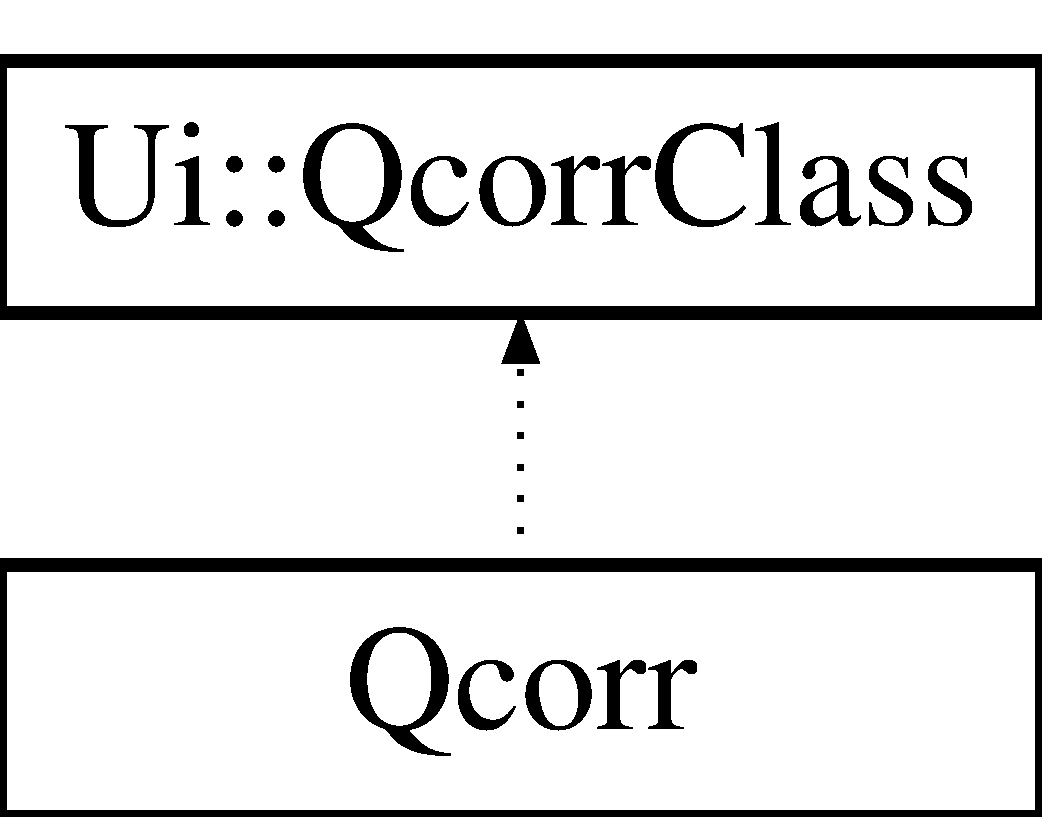
\includegraphics[height=2cm]{classQcorr}
\end{center}
\end{figure}
\subsection*{Public Member Functions}
\begin{CompactItemize}
\item 
\hypertarget{classQcorr_3b5d03aed21bfd00497ff265d898e45b}{
\hyperlink{classQcorr_3b5d03aed21bfd00497ff265d898e45b}{Qcorr} (QWidget $\ast$parent=0)}
\label{classQcorr_3b5d03aed21bfd00497ff265d898e45b}

\begin{CompactList}\small\item\em Constructor of the \hyperlink{classQcorr}{Qcorr} class. \item\end{CompactList}\item 
\hypertarget{classQcorr_c228e26878cd0b63b162f1680ab4f4fd}{
\hyperlink{classQcorr_c228e26878cd0b63b162f1680ab4f4fd}{$\sim$Qcorr} ()}
\label{classQcorr_c228e26878cd0b63b162f1680ab4f4fd}

\begin{CompactList}\small\item\em Destructor: House keeping that should be done when the \hyperlink{classQcorr}{Qcorr} main window is closed -- specifically, it closes the controlsWindow;. \item\end{CompactList}\end{CompactItemize}
\subsection*{Private Slots}
\begin{CompactItemize}
\item 
\hypertarget{classQcorr_395de1dc21d85fa766fb6558c5e302e5}{
void \hyperlink{classQcorr_395de1dc21d85fa766fb6558c5e302e5}{closeWindows} ()}
\label{classQcorr_395de1dc21d85fa766fb6558c5e302e5}

\begin{CompactList}\small\item\em Q\_\-SLOT that closes the main \hyperlink{classQcorr}{Qcorr} window and the controls Window;. \item\end{CompactList}\item 
\hypertarget{classQcorr_01b57fcc6bedf40f5c175c3fb4667a94}{
void \hyperlink{classQcorr_01b57fcc6bedf40f5c175c3fb4667a94}{showControlsWindow} ()}
\label{classQcorr_01b57fcc6bedf40f5c175c3fb4667a94}

\begin{CompactList}\small\item\em Q\_\-SLOT that shows the controls window and raises it to the foreground if already open. \item\end{CompactList}\item 
\hypertarget{classQcorr_db32e7bfe6afb84f306a9eb5bcd9b322}{
void \hyperlink{classQcorr_db32e7bfe6afb84f306a9eb5bcd9b322}{browseLeftImage} ()}
\label{classQcorr_db32e7bfe6afb84f306a9eb5bcd9b322}

\begin{CompactList}\small\item\em Q\_\-SLOT that allows to browse and load an image on the left panel. \item\end{CompactList}\item 
\hypertarget{classQcorr_60583105115d8d14c5fa2a959dc0f285}{
void \hyperlink{classQcorr_60583105115d8d14c5fa2a959dc0f285}{browseRightImage} ()}
\label{classQcorr_60583105115d8d14c5fa2a959dc0f285}

\begin{CompactList}\small\item\em Q\_\-SLOT that allows to browse and load an image on the right panel. \item\end{CompactList}\item 
\hypertarget{classQcorr_3f27a3e9b548f80998a0266c9c4165a8}{
void \hyperlink{classQcorr_3f27a3e9b548f80998a0266c9c4165a8}{changeMouse} ()}
\label{classQcorr_3f27a3e9b548f80998a0266c9c4165a8}

\begin{CompactList}\small\item\em Q\_\-SLOT used to change the mouse pointer according to the current operation mode. \item\end{CompactList}\item 
\hypertarget{classQcorr_3275244fd6183a4fef92b85578fea864}{
void \hyperlink{classQcorr_3275244fd6183a4fef92b85578fea864}{viewMap} ()}
\label{classQcorr_3275244fd6183a4fef92b85578fea864}

\begin{CompactList}\small\item\em Q\_\-SLOT that selectively provides the appropriate existent map of results from correlation (template matching) or pixel disparity. \item\end{CompactList}\item 
\hypertarget{classQcorr_f71bf39d4955ab90b859e8137b6e0761}{
void \hyperlink{classQcorr_f71bf39d4955ab90b859e8137b6e0761}{operate} ()}
\label{classQcorr_f71bf39d4955ab90b859e8137b6e0761}

\begin{CompactList}\small\item\em Q\_\-SLOT that starts the chosen operation according to the mode chosen, either template matching or disparity finder. \item\end{CompactList}\item 
\hypertarget{classQcorr_d6e0fb9461faffd01afbf62e1a0be4c3}{
void \hyperlink{classQcorr_d6e0fb9461faffd01afbf62e1a0be4c3}{abortOperation} ()}
\label{classQcorr_d6e0fb9461faffd01afbf62e1a0be4c3}

\begin{CompactList}\small\item\em Q\_\-SLOT triggers the flag to abort the current operation. \item\end{CompactList}\end{CompactItemize}
\subsection*{Private Member Functions}
\begin{CompactItemize}
\item 
void \hyperlink{classQcorr_925b0715143a0afa981851547f8b9256}{displayImage} (QImage $\ast$image, QLabel $\ast$label)
\begin{CompactList}\small\item\em Displays any QImage on a Qlabel. \item\end{CompactList}\item 
void \hyperlink{classQcorr_fddb022a6024a32be3b47016308d6c50}{displayImageLabel} (QImage $\ast$image, \hyperlink{classImgLabel}{ImgLabel} $\ast$label)
\begin{CompactList}\small\item\em Displays the reference image on the left panel's label. which is a sub-classed widget. \item\end{CompactList}\item 
\hypertarget{classQcorr_54af608880477563fa8ebcb0d066b447}{
void \hyperlink{classQcorr_54af608880477563fa8ebcb0d066b447}{createActions} ()}
\label{classQcorr_54af608880477563fa8ebcb0d066b447}

\begin{CompactList}\small\item\em Sets up actions and Q\_\-SIGNAL-Q\_\-SLOT connections. \item\end{CompactList}\item 
void \hyperlink{classQcorr_2de6d6969bdf48b225acc5ebbae063f7}{setEnableActions} (bool bEnable)
\begin{CompactList}\small\item\em Enables/Disables operation modes actions related widgets. \item\end{CompactList}\item 
\hypertarget{classQcorr_17beb7cf946cdd82f587e3b4e5ee7f19}{
void \hyperlink{classQcorr_17beb7cf946cdd82f587e3b4e5ee7f19}{setImageLabels} ()}
\label{classQcorr_17beb7cf946cdd82f587e3b4e5ee7f19}

\begin{CompactList}\small\item\em Instantiates label widgets and initializes other member variables pertinent to the overall GUI functionality of the main window itself. \item\end{CompactList}\item 
\hypertarget{classQcorr_78c77e6843a6413dbf2de14ecfd4d1d8}{
void \hyperlink{classQcorr_78c77e6843a6413dbf2de14ecfd4d1d8}{showEStop} ()}
\label{classQcorr_78c77e6843a6413dbf2de14ecfd4d1d8}

\begin{CompactList}\small\item\em emergency stop to abort the disparity operation process \item\end{CompactList}\item 
\hypertarget{classQcorr_ce91b9d83b34887735737323bac5431e}{
void \hyperlink{classQcorr_ce91b9d83b34887735737323bac5431e}{correlate} ()}
\label{classQcorr_ce91b9d83b34887735737323bac5431e}

\begin{CompactList}\small\item\em Performs template matching through correlation of the selected template against the target image. It calls \hyperlink{classQcorr_05dcc1b0be4596b355df235264180da4}{findCorrelation()} with the appropriate parameters to do a single template correlation across the entire target image. \item\end{CompactList}\item 
\hypertarget{classQcorr_640ee4c76350e5886deddbf4f0d50594}{
void \hyperlink{classQcorr_640ee4c76350e5886deddbf4f0d50594}{disparity} ()}
\label{classQcorr_640ee4c76350e5886deddbf4f0d50594}

\begin{CompactList}\small\item\em Pixel-disparity finding operation. It should be mainly be used with stereo images that can get correlated row-by-row by using \hyperlink{classQcorr_05dcc1b0be4596b355df235264180da4}{findCorrelation()} with the pertinent parameters and the appropriate Q\_\-SLOT function implementation. \item\end{CompactList}\item 
float \hyperlink{classQcorr_05dcc1b0be4596b355df235264180da4}{findCorrelation} (const unsigned char $\ast$imgTarget, const int nWI, const int nHI, const int nDepthI, const unsigned char $\ast$imgTemplate, const int nWT, const int nHT, const int nDepthT, int \&rnDx, int \&rnDy, int nMethod, bool bMultires=false, int nInitialXPosition=0, int nInitialYPosition=0, int nNumberOfRows=0)
\begin{CompactList}\small\item\em Cross-correlation of target image with template image. \item\end{CompactList}\item 
float $\ast$ \hyperlink{classQcorr_d1b26ace597c0c4a0f64a0bd9576d4fc}{convertToGrayScaleFloat} (const unsigned char $\ast$pchImgOriginalBits, int nSize, int nDepth)
\begin{CompactList}\small\item\em Cast images to an 8-bit gray-scale channel of type float. \item\end{CompactList}\item 
\hypertarget{classQcorr_bdd5c95c41d1103249d54c1ce34eecb2}{
void \hyperlink{classQcorr_bdd5c95c41d1103249d54c1ce34eecb2}{updateStatusLabelWithDisparityInfo} ()}
\label{classQcorr_bdd5c95c41d1103249d54c1ce34eecb2}

\begin{CompactList}\small\item\em Updates Status Bar with Information about parameters for the disparity operation. \item\end{CompactList}\item 
bool \hyperlink{classQcorr_87229fc918fa4011e96fbadb325fd52e}{fileDumpQImage} (const QString \&fileName)
\begin{CompactList}\small\item\em Used for testing and investing the bits stored in QImages or other Qt Widgets. \item\end{CompactList}\end{CompactItemize}
\subsection*{Private Attributes}
\begin{CompactItemize}
\item 
\hypertarget{classQcorr_53798525ce189307cf597e71aabca91b}{
int \hyperlink{classQcorr_53798525ce189307cf597e71aabca91b}{m\_\-nXCorrelationCoordinate}}
\label{classQcorr_53798525ce189307cf597e71aabca91b}

\begin{CompactList}\small\item\em the resulting x-coordinate match obtained from correlation of a template against a target \item\end{CompactList}\item 
\hypertarget{classQcorr_29f34cc7b765d5a64856696c48bfc191}{
int \hyperlink{classQcorr_29f34cc7b765d5a64856696c48bfc191}{m\_\-nYCorrelationCoordinate}}
\label{classQcorr_29f34cc7b765d5a64856696c48bfc191}

\begin{CompactList}\small\item\em the resulting y-coordinate match obtained from correlation of a template against a target \item\end{CompactList}\item 
\hypertarget{classQcorr_6509fcbf4cd8925aa109cc53e638b69a}{
\hyperlink{classCorrMethod}{CorrMethod} $\ast$ \hyperlink{classQcorr_6509fcbf4cd8925aa109cc53e638b69a}{m\_\-corrMethodDialog}}
\label{classQcorr_6509fcbf4cd8925aa109cc53e638b69a}

\begin{CompactList}\small\item\em Dialog Box to choose a correlation method. \item\end{CompactList}\item 
\hypertarget{classQcorr_5b43654ac42b41b945cd58ce62b18ed0}{
\hyperlink{classControlsWindow}{ControlsWindow} $\ast$ \hyperlink{classQcorr_5b43654ac42b41b945cd58ce62b18ed0}{m\_\-controlsWindow}}
\label{classQcorr_5b43654ac42b41b945cd58ce62b18ed0}

\begin{CompactList}\small\item\em Dialog Box to modify correlation parameters such as template size and scan interval. \item\end{CompactList}\item 
\hypertarget{classQcorr_3430716ddbe203f677095c163da87f86}{
QString \hyperlink{classQcorr_3430716ddbe203f677095c163da87f86}{initialName}}
\label{classQcorr_3430716ddbe203f677095c163da87f86}

\begin{CompactList}\small\item\em String that saves the path for the first file image that has been loaded. \item\end{CompactList}\item 
\hypertarget{classQcorr_e8bdd4be8a0c3023be34a1301b28c913}{
QImage $\ast$ \hyperlink{classQcorr_e8bdd4be8a0c3023be34a1301b28c913}{m\_\-leftImage}}
\label{classQcorr_e8bdd4be8a0c3023be34a1301b28c913}

\begin{CompactList}\small\item\em Left Panel's Image (a.k.a. \char`\"{}reference image\char`\"{} when performing template matching through correlation). \item\end{CompactList}\item 
\hypertarget{classQcorr_ae1695d731f191c694186e00b96f469e}{
QImage $\ast$ \hyperlink{classQcorr_ae1695d731f191c694186e00b96f469e}{m\_\-rightImage}}
\label{classQcorr_ae1695d731f191c694186e00b96f469e}

\begin{CompactList}\small\item\em Right Panel's Image (a.k.a \char`\"{}target image\char`\"{}). \item\end{CompactList}\item 
\hypertarget{classQcorr_5594d939890f10991da0009e4c32bea3}{
QImage $\ast$ \hyperlink{classQcorr_5594d939890f10991da0009e4c32bea3}{m\_\-templateImage}}
\label{classQcorr_5594d939890f10991da0009e4c32bea3}

\begin{CompactList}\small\item\em Template Image that is selected from the reference image (in the left panel) that will be matched against. \item\end{CompactList}\item 
\hypertarget{classQcorr_c7dc2785613864bea2d8bb0b5f009f36}{
QImage $\ast$ \hyperlink{classQcorr_c7dc2785613864bea2d8bb0b5f009f36}{m\_\-corrMapImage}}
\label{classQcorr_c7dc2785613864bea2d8bb0b5f009f36}

\begin{CompactList}\small\item\em Correlation Map resulting from the Template Matching action. \item\end{CompactList}\item 
\hypertarget{classQcorr_731915641051962d6a03a31b772640d4}{
QImage $\ast$ \hyperlink{classQcorr_731915641051962d6a03a31b772640d4}{m\_\-disparityMapImage}}
\label{classQcorr_731915641051962d6a03a31b772640d4}

\begin{CompactList}\small\item\em Disparity Map that results from the pixel disparities found between the left and right images. \item\end{CompactList}\item 
\hypertarget{classQcorr_cadb3032fbf41f8f1b27067c2784efef}{
\hyperlink{classImgLabel}{ImgLabel} $\ast$ \hyperlink{classQcorr_cadb3032fbf41f8f1b27067c2784efef}{m\_\-leftImage\_\-label}}
\label{classQcorr_cadb3032fbf41f8f1b27067c2784efef}

\begin{CompactList}\small\item\em label used to display the left image. This is sub-classed widget implemented with the functionality of allowing template selection by a rectangular rubber-band \item\end{CompactList}\item 
\hypertarget{classQcorr_8d1e1ab866a811003c435c45de1e958e}{
\hyperlink{classTargetImgLabel}{TargetImgLabel} $\ast$ \hyperlink{classQcorr_8d1e1ab866a811003c435c45de1e958e}{m\_\-targetImage\_\-label}}
\label{classQcorr_8d1e1ab866a811003c435c45de1e958e}

\begin{CompactList}\small\item\em a sub-classed label widget implemented with the purpose of displaying the target image in the right panel with added functionality such as the visualization of the found match \item\end{CompactList}\item 
\hypertarget{classQcorr_1bf4a70aa6c4e171f2e0613109bb57e9}{
QLabel $\ast$ \hyperlink{classQcorr_1bf4a70aa6c4e171f2e0613109bb57e9}{m\_\-status\_\-label}}
\label{classQcorr_1bf4a70aa6c4e171f2e0613109bb57e9}

\begin{CompactList}\small\item\em status label that updates the mouse-pointer's position coordinates as it moves and selects templates. It also provides other types of information when required. \item\end{CompactList}\item 
\hypertarget{classQcorr_fa1be55387e39ce5b81e72ecab75b5bc}{
QVector$<$ QRgb $>$ $\ast$ \hyperlink{classQcorr_fa1be55387e39ce5b81e72ecab75b5bc}{m\_\-grayColorTab}}
\label{classQcorr_fa1be55387e39ce5b81e72ecab75b5bc}

\begin{CompactList}\small\item\em 8-bit gray-scale color table \item\end{CompactList}\item 
\hypertarget{classQcorr_795a9f4f9805a241f55c59a0a520f3d4}{
QVector$<$ QRgb $>$ $\ast$ \hyperlink{classQcorr_795a9f4f9805a241f55c59a0a520f3d4}{m\_\-greenColorTab}}
\label{classQcorr_795a9f4f9805a241f55c59a0a520f3d4}

\begin{CompactList}\small\item\em 8-bit green-scale color table \item\end{CompactList}\item 
\hypertarget{classQcorr_8a7f00160ae46441cef038149cf28bdc}{
QPoint \hyperlink{classQcorr_8a7f00160ae46441cef038149cf28bdc}{m\_\-matchingPoint}}
\label{classQcorr_8a7f00160ae46441cef038149cf28bdc}

\begin{CompactList}\small\item\em upper-left corner point where the correlation match was found \item\end{CompactList}\item 
\hypertarget{classQcorr_bc48bdd2110cfdaf7b98dde1cdf42f18}{
QSize \hyperlink{classQcorr_bc48bdd2110cfdaf7b98dde1cdf42f18}{m\_\-templateSize}}
\label{classQcorr_bc48bdd2110cfdaf7b98dde1cdf42f18}

\begin{CompactList}\small\item\em the current template's size as a QSize object \item\end{CompactList}\item 
\hypertarget{classQcorr_3a964df80562c062d5f1f4f6cbf841bb}{
QActionGroup $\ast$ \hyperlink{classQcorr_3a964df80562c062d5f1f4f6cbf841bb}{modes\_\-actionGroup}}
\label{classQcorr_3a964df80562c062d5f1f4f6cbf841bb}

\begin{CompactList}\small\item\em group of menu actions for the mode of operation. \item\end{CompactList}\item 
\hypertarget{classQcorr_496beab48555a8c9abbd6f6aa48e52fb}{
QDialogButtonBox $\ast$ \hyperlink{classQcorr_496beab48555a8c9abbd6f6aa48e52fb}{m\_\-eStopDialog}}
\label{classQcorr_496beab48555a8c9abbd6f6aa48e52fb}

\begin{CompactList}\small\item\em A dialogue to stop the current correlation process. \item\end{CompactList}\item 
\hypertarget{classQcorr_b5325b11a64e24eeb6b9bdc27a77d0ad}{
bool \hyperlink{classQcorr_b5325b11a64e24eeb6b9bdc27a77d0ad}{m\_\-bHasLeftImage}}
\label{classQcorr_b5325b11a64e24eeb6b9bdc27a77d0ad}

\begin{CompactList}\small\item\em indicates that an image is loaded in the left panel \item\end{CompactList}\item 
\hypertarget{classQcorr_a4afa1daa72ecf6caae74f6ced4ec251}{
bool \hyperlink{classQcorr_a4afa1daa72ecf6caae74f6ced4ec251}{m\_\-bHasRightImage}}
\label{classQcorr_a4afa1daa72ecf6caae74f6ced4ec251}

\begin{CompactList}\small\item\em indicates that an image is loaded in the right panel \item\end{CompactList}\item 
\hypertarget{classQcorr_40e40bfd5cc79d8abf6e7b41465f440e}{
bool \hyperlink{classQcorr_40e40bfd5cc79d8abf6e7b41465f440e}{m\_\-bHasCorrMap}}
\label{classQcorr_40e40bfd5cc79d8abf6e7b41465f440e}

\begin{CompactList}\small\item\em indicates that a correlation map exists \item\end{CompactList}\item 
\hypertarget{classQcorr_42ef5dadd6c1ff9f560de8cb1f43c2c6}{
bool \hyperlink{classQcorr_42ef5dadd6c1ff9f560de8cb1f43c2c6}{m\_\-bHasDisparityMap}}
\label{classQcorr_42ef5dadd6c1ff9f560de8cb1f43c2c6}

\begin{CompactList}\small\item\em indicates that a disparity map exists \item\end{CompactList}\item 
\hypertarget{classQcorr_db31096514465f8c4a1993345d98f1eb}{
bool \hyperlink{classQcorr_db31096514465f8c4a1993345d98f1eb}{m\_\-bEstop}}
\label{classQcorr_db31096514465f8c4a1993345d98f1eb}

\begin{CompactList}\small\item\em emergency stop for the \item\end{CompactList}\item 
\hypertarget{classQcorr_b07379fbbd7be906023eb5ec4d555931}{
int \hyperlink{classQcorr_b07379fbbd7be906023eb5ec4d555931}{m\_\-nScanInterval}}
\label{classQcorr_b07379fbbd7be906023eb5ec4d555931}

\begin{CompactList}\small\item\em interval of scan traversal by the template \item\end{CompactList}\end{CompactItemize}
\subsection*{Friends}
\begin{CompactItemize}
\item 
class \hyperlink{classQcorr_5b4b2caf4c596b601dd096785e4a32b9}{ImgLabel}
\begin{CompactList}\small\item\em the \hyperlink{classImgLabel}{ImgLabel} class is a friend of \hyperlink{classQcorr}{Qcorr} in order to make all members of \hyperlink{classQcorr}{Qcorr} accessible by an \hyperlink{classImgLabel}{ImgLabel} object \item\end{CompactList}\item 
class \hyperlink{classQcorr_ce49e9a34b2d2df1e7683be4cacba1d8}{ControlsWindow}
\begin{CompactList}\small\item\em allows to modify parameters for the correlation operations, such as template size and scan interval. This class is a friend of \hyperlink{classQcorr}{Qcorr}. \item\end{CompactList}\end{CompactItemize}


\subsection{Detailed Description}
A Digital Image Correlation Program (Template Matching and Pixel Disparity Finder) implemented in QT4. 

This class combines all other sub-classed QWidgets implemented throughout the program. The main correlation used in the \char`\"{}Template matching\char`\"{} and \char`\"{}Disparity Finder\char`\"{} modes rely strongly in the functionality implemented in this class through the procedure \hyperlink{classQcorr_d1b26ace597c0c4a0f64a0bd9576d4fc}{convertToGrayScaleFloat()}

\begin{Desc}
\item[Note:]Correlation is performed on gray-scale (1 channel image) that are computed in this procedure through the \hyperlink{classQcorr_d1b26ace597c0c4a0f64a0bd9576d4fc}{convertToGrayScaleFloat()} function.\end{Desc}
\begin{Desc}
\item[Compile-time dependencies]\begin{itemize}
\item The QT4 Framework\item g++\end{itemize}
\end{Desc}
\begin{Desc}
\item[\hyperlink{bug__bug000001}{Bug}]\begin{itemize}
\item Perhaps a few around the rubberBand functionality, and others not noticed yet.\end{itemize}
\end{Desc}
\begin{Desc}
\item[\hyperlink{todo__todo000001}{Todo}]\begin{itemize}
\item Use pyramids method for faster correlation\item Better disparity map implementation\item Spacebar opens full screen mode on image.\end{itemize}
\end{Desc}
\begin{Desc}
\item[Authors:]Carlos Jaramillo 

Joel Gonzalez \end{Desc}


Definition at line 52 of file qcorr.h.

\subsection{Member Function Documentation}
\hypertarget{classQcorr_d1b26ace597c0c4a0f64a0bd9576d4fc}{
\index{Qcorr@{Qcorr}!convertToGrayScaleFloat@{convertToGrayScaleFloat}}
\index{convertToGrayScaleFloat@{convertToGrayScaleFloat}!Qcorr@{Qcorr}}
\subsubsection[{convertToGrayScaleFloat}]{\setlength{\rightskip}{0pt plus 5cm}float $\ast$ Qcorr::convertToGrayScaleFloat (const unsigned char $\ast$ {\em pchImgOriginalBits}, \/  int {\em nSize}, \/  int {\em nDepth})\hspace{0.3cm}{\tt  \mbox{[}private\mbox{]}}}}
\label{classQcorr_d1b26ace597c0c4a0f64a0bd9576d4fc}


Cast images to an 8-bit gray-scale channel of type float. 

\begin{Desc}
\item[Parameters:]
\begin{description}
\item[{\em pchImgOriginalBits}]Buffer of unsigned characters as the source image \item[{\em nSize}]Number of pixels in the source image \item[{\em nDepth}]Pixel depth of the source image \end{description}
\end{Desc}
\begin{Desc}
\item[Returns:]the correlation number computed by method (directly). Additionally, the (dx,dy) offset of the template for which there exists a best match. \end{Desc}


Definition at line 1296 of file qcorr.cpp.

Referenced by findCorrelation().\hypertarget{classQcorr_925b0715143a0afa981851547f8b9256}{
\index{Qcorr@{Qcorr}!displayImage@{displayImage}}
\index{displayImage@{displayImage}!Qcorr@{Qcorr}}
\subsubsection[{displayImage}]{\setlength{\rightskip}{0pt plus 5cm}void Qcorr::displayImage (QImage $\ast$ {\em image}, \/  QLabel $\ast$ {\em label})\hspace{0.3cm}{\tt  \mbox{[}private\mbox{]}}}}
\label{classQcorr_925b0715143a0afa981851547f8b9256}


Displays any QImage on a Qlabel. 

\begin{Desc}
\item[Parameters:]
\begin{description}
\item[{\em image}]Pointer to a QImage instance \item[{\em label}]Pointer to a QLabel instance \end{description}
\end{Desc}


Definition at line 1279 of file qcorr.cpp.\hypertarget{classQcorr_fddb022a6024a32be3b47016308d6c50}{
\index{Qcorr@{Qcorr}!displayImageLabel@{displayImageLabel}}
\index{displayImageLabel@{displayImageLabel}!Qcorr@{Qcorr}}
\subsubsection[{displayImageLabel}]{\setlength{\rightskip}{0pt plus 5cm}void Qcorr::displayImageLabel (QImage $\ast$ {\em image}, \/  {\bf ImgLabel} $\ast$ {\em label})\hspace{0.3cm}{\tt  \mbox{[}private\mbox{]}}}}
\label{classQcorr_fddb022a6024a32be3b47016308d6c50}


Displays the reference image on the left panel's label. which is a sub-classed widget. 

\begin{Desc}
\item[Parameters:]
\begin{description}
\item[{\em image}]Pointer to a QImage instance \item[{\em label}]Pointer to a \hyperlink{classImgLabel}{ImgLabel} class instance \end{description}
\end{Desc}


Definition at line 1286 of file qcorr.cpp.

References ImgLabel::m\_\-labelLowerRightCornerPoint.

Referenced by browseLeftImage().\hypertarget{classQcorr_87229fc918fa4011e96fbadb325fd52e}{
\index{Qcorr@{Qcorr}!fileDumpQImage@{fileDumpQImage}}
\index{fileDumpQImage@{fileDumpQImage}!Qcorr@{Qcorr}}
\subsubsection[{fileDumpQImage}]{\setlength{\rightskip}{0pt plus 5cm}bool Qcorr::fileDumpQImage (const QString \& {\em fileName})\hspace{0.3cm}{\tt  \mbox{[}private\mbox{]}}}}
\label{classQcorr_87229fc918fa4011e96fbadb325fd52e}


Used for testing and investing the bits stored in QImages or other Qt Widgets. 

\begin{Desc}
\item[Parameters:]
\begin{description}
\item[{\em fileName}]a QString reference to the file-name as which the raw bits will be storedpchImgOriginalBits Buffer of unsigned characters as the source image \end{description}
\end{Desc}
\begin{Desc}
\item[Returns:]true if the bits were properly dumped to the specified fileName \end{Desc}


Definition at line 1353 of file qcorr.cpp.

References m\_\-rightImage.\hypertarget{classQcorr_05dcc1b0be4596b355df235264180da4}{
\index{Qcorr@{Qcorr}!findCorrelation@{findCorrelation}}
\index{findCorrelation@{findCorrelation}!Qcorr@{Qcorr}}
\subsubsection[{findCorrelation}]{\setlength{\rightskip}{0pt plus 5cm}float Qcorr::findCorrelation (const unsigned char $\ast$ {\em imgTarget}, \/  const int {\em nWI}, \/  const int {\em nHI}, \/  const int {\em nDepthI}, \/  const unsigned char $\ast$ {\em imgTemplate}, \/  const int {\em nWT}, \/  const int {\em nHT}, \/  const int {\em nDepthT}, \/  int \& {\em rnDx}, \/  int \& {\em rnDy}, \/  int {\em nMethod}, \/  bool {\em bMultires} = {\tt false}, \/  int {\em nInitialXPosition} = {\tt 0}, \/  int {\em nInitialYPosition} = {\tt 0}, \/  int {\em nNumberOfRows} = {\tt 0})\hspace{0.3cm}{\tt  \mbox{[}private\mbox{]}}}}
\label{classQcorr_05dcc1b0be4596b355df235264180da4}


Cross-correlation of target image with template image. 

\begin{Desc}
\item[Note:]Correlation is performed on gray-scale (1 channel image) that are computed in this procedure through the \hyperlink{classQcorr_d1b26ace597c0c4a0f64a0bd9576d4fc}{convertToGrayScaleFloat()} function. \end{Desc}
\begin{Desc}
\item[Parameters:]
\begin{description}
\item[{\em imgTarget}]Buffer of unsigned characters containing the target image where correlation match is to be found \item[{\em nWI}]Width of target image \item[{\em nHI}]Height of target image \item[{\em nDepthI}]Pixel depth of target image \item[{\em imgTemplate}]Buffer of unsigned characters containing the template image \item[{\em nWT}]Width of target image \item[{\em nHT}]Height of target image \item[{\em nDepthT}]Pixel depth of target image \item[{\em rnDx}]x-coordinate where the highest level of correlation match is found (top-left corner of the match) \item[{\em rnDy}]y-coordinate where the highest level of correlation match is found (top-left corner of the match) \item[{\em nMethod}]Determines the selected method to be used in the correlation process. The method is a globally defined enumeration. The available methods are:\begin{itemize}
\item CROSS\_\-CORR (cross correlation): \[ C(u,v) = \frac {\sum{\left\{T(x,y) * I(x-u,y-v)\right\}}} {\sqrt{ \sum{I(x-u,y-v)^2}}} \]\item SUM\_\-SQ\_\-DIFF (sum of squared differences): \[ C(u,v) = \frac {\sum{\left\{T(x,y)-I(x-u,y-v)\right\}^2}} {\sqrt{\sum{I(x-u,y-v)^2}}} \]\item CORR\_\-COEFF (correlation coefficient): \[ C(u,v) = \frac {\sum{\left\{(T(x,y)-T_{avg}) * (I(x-u,y-v)-I_{avg})\right\}}} {\sqrt{\sum{(T(x,y)-T_{avg})^2} * \sum{(I(x-u,y-v)-I_{avg})^2}}} \] Remark: The square root of the sum of the squares (RSS) is being used to calculate the aggregate accuracy of a measurement when the accuracies of the all the measuring devices are known. The average accuracy is not merely the arithmetic average of the accuracies (or uncertainties), nor is it the sum of them. Note how the RSS result in this case is greater than the largest of the values under the radical.\end{itemize}
\item[{\em bMultires}]Determines if multiresolution correlation should be applied, by making use of image pyramids. With multiresoltion, the correlation can be determined faster than direct correlation. Default is false. \item[{\em nInitialXPosition}]Indicates the x-coordinate of the pixel on the target image where correlation should start. Default is 0 \item[{\em nInitialYPosition}]Indicates the y-coordinate of the pixel on the target image where correlation should start. Default is 0 \item[{\em nNumberOfRows}]Indicates the number of rows on the target image to be scanned. Default is 0, which means all of them. \end{description}
\end{Desc}
\begin{Desc}
\item[Returns:]a float array resulting from the conversion of the source image into an 8-bit gray-scale image. \end{Desc}


Definition at line 643 of file qcorr.cpp.

References convertToGrayScaleFloat(), m\_\-bEstop, m\_\-bHasCorrMap, m\_\-corrMapImage, and m\_\-grayColorTab.

Referenced by correlate(), and disparity().\hypertarget{classQcorr_2de6d6969bdf48b225acc5ebbae063f7}{
\index{Qcorr@{Qcorr}!setEnableActions@{setEnableActions}}
\index{setEnableActions@{setEnableActions}!Qcorr@{Qcorr}}
\subsubsection[{setEnableActions}]{\setlength{\rightskip}{0pt plus 5cm}void Qcorr::setEnableActions (bool {\em bEnable})\hspace{0.3cm}{\tt  \mbox{[}private\mbox{]}}}}
\label{classQcorr_2de6d6969bdf48b225acc5ebbae063f7}


Enables/Disables operation modes actions related widgets. 

\begin{Desc}
\item[Parameters:]
\begin{description}
\item[{\em bEnable}]boolean flag to enable or disable the operation mode's actions widgets as well as the related widgets such as, start\_\-pushButton and controls\_\-pushButton \end{description}
\end{Desc}


Definition at line 167 of file qcorr.cpp.

References changeMouse().

Referenced by browseLeftImage(), and browseRightImage().

\subsection{Friends And Related Function Documentation}
\hypertarget{classQcorr_ce49e9a34b2d2df1e7683be4cacba1d8}{
\index{Qcorr@{Qcorr}!ControlsWindow@{ControlsWindow}}
\index{ControlsWindow@{ControlsWindow}!Qcorr@{Qcorr}}
\subsubsection[{ControlsWindow}]{\setlength{\rightskip}{0pt plus 5cm}friend class {\bf ControlsWindow}\hspace{0.3cm}{\tt  \mbox{[}friend\mbox{]}}}}
\label{classQcorr_ce49e9a34b2d2df1e7683be4cacba1d8}


allows to modify parameters for the correlation operations, such as template size and scan interval. This class is a friend of \hyperlink{classQcorr}{Qcorr}. 

\hyperlink{classControlsWindow}{ControlsWindow} 

Definition at line 87 of file qcorr.h.

Referenced by setImageLabels().\hypertarget{classQcorr_5b4b2caf4c596b601dd096785e4a32b9}{
\index{Qcorr@{Qcorr}!ImgLabel@{ImgLabel}}
\index{ImgLabel@{ImgLabel}!Qcorr@{Qcorr}}
\subsubsection[{ImgLabel}]{\setlength{\rightskip}{0pt plus 5cm}friend class {\bf ImgLabel}\hspace{0.3cm}{\tt  \mbox{[}friend\mbox{]}}}}
\label{classQcorr_5b4b2caf4c596b601dd096785e4a32b9}


the \hyperlink{classImgLabel}{ImgLabel} class is a friend of \hyperlink{classQcorr}{Qcorr} in order to make all members of \hyperlink{classQcorr}{Qcorr} accessible by an \hyperlink{classImgLabel}{ImgLabel} object 

\hyperlink{classImgLabel}{ImgLabel} 

Definition at line 82 of file qcorr.h.

Referenced by setImageLabels().

The documentation for this class was generated from the following files:\begin{CompactItemize}
\item 
src/qcorr.h\item 
src/qcorr.cpp\end{CompactItemize}

\hypertarget{classQcorr}{
\section{Qcorr Class Reference}
\label{classQcorr}\index{Qcorr@{Qcorr}}
}
A Digital Image Correlation Program (Template Matching and Pixel Disparity Finder) implemented in QT4.  


{\tt \#include $<$src/qcorr.h$>$}

Inheritance diagram for Qcorr::\begin{figure}[H]
\begin{center}
\leavevmode
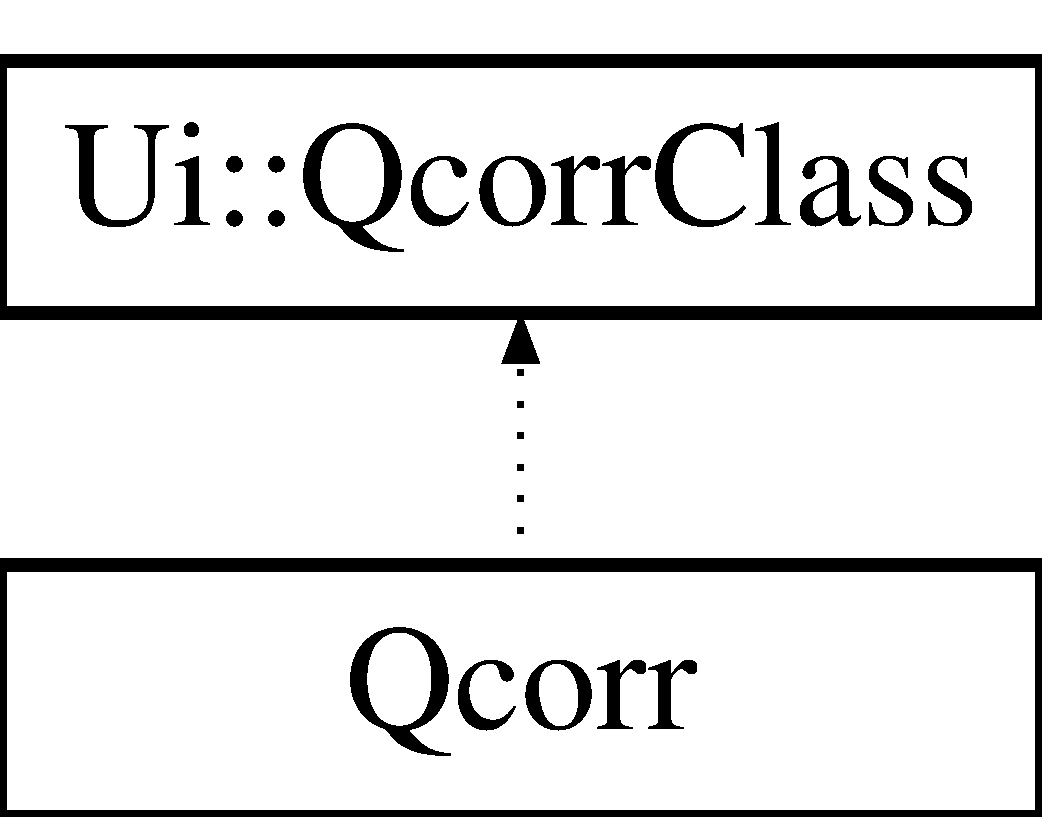
\includegraphics[height=2cm]{classQcorr}
\end{center}
\end{figure}
\subsection*{Public Member Functions}
\begin{CompactItemize}
\item 
\hypertarget{classQcorr_3b5d03aed21bfd00497ff265d898e45b}{
\hyperlink{classQcorr_3b5d03aed21bfd00497ff265d898e45b}{Qcorr} (QWidget $\ast$parent=0)}
\label{classQcorr_3b5d03aed21bfd00497ff265d898e45b}

\begin{CompactList}\small\item\em Constructor of the \hyperlink{classQcorr}{Qcorr} class. \item\end{CompactList}\item 
\hypertarget{classQcorr_c228e26878cd0b63b162f1680ab4f4fd}{
\hyperlink{classQcorr_c228e26878cd0b63b162f1680ab4f4fd}{$\sim$Qcorr} ()}
\label{classQcorr_c228e26878cd0b63b162f1680ab4f4fd}

\begin{CompactList}\small\item\em Destructor: House keeping that should be done when the \hyperlink{classQcorr}{Qcorr} main window is closed -- specifically, it closes the controlsWindow;. \item\end{CompactList}\end{CompactItemize}
\subsection*{Private Slots}
\begin{CompactItemize}
\item 
\hypertarget{classQcorr_395de1dc21d85fa766fb6558c5e302e5}{
void \hyperlink{classQcorr_395de1dc21d85fa766fb6558c5e302e5}{closeWindows} ()}
\label{classQcorr_395de1dc21d85fa766fb6558c5e302e5}

\begin{CompactList}\small\item\em Q\_\-SLOT that closes the main \hyperlink{classQcorr}{Qcorr} window and the controls Window;. \item\end{CompactList}\item 
\hypertarget{classQcorr_01b57fcc6bedf40f5c175c3fb4667a94}{
void \hyperlink{classQcorr_01b57fcc6bedf40f5c175c3fb4667a94}{showControlsWindow} ()}
\label{classQcorr_01b57fcc6bedf40f5c175c3fb4667a94}

\begin{CompactList}\small\item\em Q\_\-SLOT that shows the controls window and raises it to the foreground if already open. \item\end{CompactList}\item 
\hypertarget{classQcorr_db32e7bfe6afb84f306a9eb5bcd9b322}{
void \hyperlink{classQcorr_db32e7bfe6afb84f306a9eb5bcd9b322}{browseLeftImage} ()}
\label{classQcorr_db32e7bfe6afb84f306a9eb5bcd9b322}

\begin{CompactList}\small\item\em Q\_\-SLOT that allows to browse and load an image on the left panel. \item\end{CompactList}\item 
\hypertarget{classQcorr_60583105115d8d14c5fa2a959dc0f285}{
void \hyperlink{classQcorr_60583105115d8d14c5fa2a959dc0f285}{browseRightImage} ()}
\label{classQcorr_60583105115d8d14c5fa2a959dc0f285}

\begin{CompactList}\small\item\em Q\_\-SLOT that allows to browse and load an image on the right panel. \item\end{CompactList}\item 
\hypertarget{classQcorr_3f27a3e9b548f80998a0266c9c4165a8}{
void \hyperlink{classQcorr_3f27a3e9b548f80998a0266c9c4165a8}{changeMouse} ()}
\label{classQcorr_3f27a3e9b548f80998a0266c9c4165a8}

\begin{CompactList}\small\item\em Q\_\-SLOT used to change the mouse pointer according to the current operation mode. \item\end{CompactList}\item 
\hypertarget{classQcorr_3275244fd6183a4fef92b85578fea864}{
void \hyperlink{classQcorr_3275244fd6183a4fef92b85578fea864}{viewMap} ()}
\label{classQcorr_3275244fd6183a4fef92b85578fea864}

\begin{CompactList}\small\item\em Q\_\-SLOT that selectively provides the appropriate existent map of results from correlation (template matching) or pixel disparity. \item\end{CompactList}\item 
\hypertarget{classQcorr_f71bf39d4955ab90b859e8137b6e0761}{
void \hyperlink{classQcorr_f71bf39d4955ab90b859e8137b6e0761}{operate} ()}
\label{classQcorr_f71bf39d4955ab90b859e8137b6e0761}

\begin{CompactList}\small\item\em Q\_\-SLOT that starts the chosen operation according to the mode chosen, either template matching or disparity finder. \item\end{CompactList}\item 
\hypertarget{classQcorr_d6e0fb9461faffd01afbf62e1a0be4c3}{
void \hyperlink{classQcorr_d6e0fb9461faffd01afbf62e1a0be4c3}{abortOperation} ()}
\label{classQcorr_d6e0fb9461faffd01afbf62e1a0be4c3}

\begin{CompactList}\small\item\em Q\_\-SLOT triggers the flag to abort the current operation. \item\end{CompactList}\end{CompactItemize}
\subsection*{Private Member Functions}
\begin{CompactItemize}
\item 
void \hyperlink{classQcorr_925b0715143a0afa981851547f8b9256}{displayImage} (QImage $\ast$image, QLabel $\ast$label)
\begin{CompactList}\small\item\em Displays any QImage on a Qlabel. \item\end{CompactList}\item 
void \hyperlink{classQcorr_fddb022a6024a32be3b47016308d6c50}{displayImageLabel} (QImage $\ast$image, \hyperlink{classImgLabel}{ImgLabel} $\ast$label)
\begin{CompactList}\small\item\em Displays the reference image on the left panel's label. which is a sub-classed widget. \item\end{CompactList}\item 
\hypertarget{classQcorr_54af608880477563fa8ebcb0d066b447}{
void \hyperlink{classQcorr_54af608880477563fa8ebcb0d066b447}{createActions} ()}
\label{classQcorr_54af608880477563fa8ebcb0d066b447}

\begin{CompactList}\small\item\em Sets up actions and Q\_\-SIGNAL-Q\_\-SLOT connections. \item\end{CompactList}\item 
void \hyperlink{classQcorr_2de6d6969bdf48b225acc5ebbae063f7}{setEnableActions} (bool bEnable)
\begin{CompactList}\small\item\em Enables/Disables operation modes actions related widgets. \item\end{CompactList}\item 
\hypertarget{classQcorr_17beb7cf946cdd82f587e3b4e5ee7f19}{
void \hyperlink{classQcorr_17beb7cf946cdd82f587e3b4e5ee7f19}{setImageLabels} ()}
\label{classQcorr_17beb7cf946cdd82f587e3b4e5ee7f19}

\begin{CompactList}\small\item\em Instantiates label widgets and initializes other member variables pertinent to the overall GUI functionality of the main window itself. \item\end{CompactList}\item 
\hypertarget{classQcorr_78c77e6843a6413dbf2de14ecfd4d1d8}{
void \hyperlink{classQcorr_78c77e6843a6413dbf2de14ecfd4d1d8}{showEStop} ()}
\label{classQcorr_78c77e6843a6413dbf2de14ecfd4d1d8}

\begin{CompactList}\small\item\em emergency stop to abort the disparity operation process \item\end{CompactList}\item 
\hypertarget{classQcorr_ce91b9d83b34887735737323bac5431e}{
void \hyperlink{classQcorr_ce91b9d83b34887735737323bac5431e}{correlate} ()}
\label{classQcorr_ce91b9d83b34887735737323bac5431e}

\begin{CompactList}\small\item\em Performs template matching through correlation of the selected template against the target image. It calls \hyperlink{classQcorr_05dcc1b0be4596b355df235264180da4}{findCorrelation()} with the appropriate parameters to do a single template correlation across the entire target image. \item\end{CompactList}\item 
\hypertarget{classQcorr_640ee4c76350e5886deddbf4f0d50594}{
void \hyperlink{classQcorr_640ee4c76350e5886deddbf4f0d50594}{disparity} ()}
\label{classQcorr_640ee4c76350e5886deddbf4f0d50594}

\begin{CompactList}\small\item\em Pixel-disparity finding operation. It should be mainly be used with stereo images that can get correlated row-by-row by using \hyperlink{classQcorr_05dcc1b0be4596b355df235264180da4}{findCorrelation()} with the pertinent parameters and the appropriate Q\_\-SLOT function implementation. \item\end{CompactList}\item 
float \hyperlink{classQcorr_05dcc1b0be4596b355df235264180da4}{findCorrelation} (const unsigned char $\ast$imgTarget, const int nWI, const int nHI, const int nDepthI, const unsigned char $\ast$imgTemplate, const int nWT, const int nHT, const int nDepthT, int \&rnDx, int \&rnDy, int nMethod, bool bMultires=false, int nInitialXPosition=0, int nInitialYPosition=0, int nNumberOfRows=0)
\begin{CompactList}\small\item\em Cross-correlation of target image with template image. \item\end{CompactList}\item 
float $\ast$ \hyperlink{classQcorr_d1b26ace597c0c4a0f64a0bd9576d4fc}{convertToGrayScaleFloat} (const unsigned char $\ast$pchImgOriginalBits, int nSize, int nDepth)
\begin{CompactList}\small\item\em Cast images to an 8-bit gray-scale channel of type float. \item\end{CompactList}\item 
\hypertarget{classQcorr_bdd5c95c41d1103249d54c1ce34eecb2}{
void \hyperlink{classQcorr_bdd5c95c41d1103249d54c1ce34eecb2}{updateStatusLabelWithDisparityInfo} ()}
\label{classQcorr_bdd5c95c41d1103249d54c1ce34eecb2}

\begin{CompactList}\small\item\em Updates Status Bar with Information about parameters for the disparity operation. \item\end{CompactList}\item 
bool \hyperlink{classQcorr_87229fc918fa4011e96fbadb325fd52e}{fileDumpQImage} (const QString \&fileName)
\begin{CompactList}\small\item\em Used for testing and investing the bits stored in QImages or other Qt Widgets. \item\end{CompactList}\end{CompactItemize}
\subsection*{Private Attributes}
\begin{CompactItemize}
\item 
\hypertarget{classQcorr_53798525ce189307cf597e71aabca91b}{
int \hyperlink{classQcorr_53798525ce189307cf597e71aabca91b}{m\_\-nXCorrelationCoordinate}}
\label{classQcorr_53798525ce189307cf597e71aabca91b}

\begin{CompactList}\small\item\em the resulting x-coordinate match obtained from correlation of a template against a target \item\end{CompactList}\item 
\hypertarget{classQcorr_29f34cc7b765d5a64856696c48bfc191}{
int \hyperlink{classQcorr_29f34cc7b765d5a64856696c48bfc191}{m\_\-nYCorrelationCoordinate}}
\label{classQcorr_29f34cc7b765d5a64856696c48bfc191}

\begin{CompactList}\small\item\em the resulting y-coordinate match obtained from correlation of a template against a target \item\end{CompactList}\item 
\hypertarget{classQcorr_6509fcbf4cd8925aa109cc53e638b69a}{
\hyperlink{classCorrMethod}{CorrMethod} $\ast$ \hyperlink{classQcorr_6509fcbf4cd8925aa109cc53e638b69a}{m\_\-corrMethodDialog}}
\label{classQcorr_6509fcbf4cd8925aa109cc53e638b69a}

\begin{CompactList}\small\item\em Dialog Box to choose a correlation method. \item\end{CompactList}\item 
\hypertarget{classQcorr_5b43654ac42b41b945cd58ce62b18ed0}{
\hyperlink{classControlsWindow}{ControlsWindow} $\ast$ \hyperlink{classQcorr_5b43654ac42b41b945cd58ce62b18ed0}{m\_\-controlsWindow}}
\label{classQcorr_5b43654ac42b41b945cd58ce62b18ed0}

\begin{CompactList}\small\item\em Dialog Box to modify correlation parameters such as template size and scan interval. \item\end{CompactList}\item 
\hypertarget{classQcorr_3430716ddbe203f677095c163da87f86}{
QString \hyperlink{classQcorr_3430716ddbe203f677095c163da87f86}{initialName}}
\label{classQcorr_3430716ddbe203f677095c163da87f86}

\begin{CompactList}\small\item\em String that saves the path for the first file image that has been loaded. \item\end{CompactList}\item 
\hypertarget{classQcorr_e8bdd4be8a0c3023be34a1301b28c913}{
QImage $\ast$ \hyperlink{classQcorr_e8bdd4be8a0c3023be34a1301b28c913}{m\_\-leftImage}}
\label{classQcorr_e8bdd4be8a0c3023be34a1301b28c913}

\begin{CompactList}\small\item\em Left Panel's Image (a.k.a. \char`\"{}reference image\char`\"{} when performing template matching through correlation). \item\end{CompactList}\item 
\hypertarget{classQcorr_ae1695d731f191c694186e00b96f469e}{
QImage $\ast$ \hyperlink{classQcorr_ae1695d731f191c694186e00b96f469e}{m\_\-rightImage}}
\label{classQcorr_ae1695d731f191c694186e00b96f469e}

\begin{CompactList}\small\item\em Right Panel's Image (a.k.a \char`\"{}target image\char`\"{}). \item\end{CompactList}\item 
\hypertarget{classQcorr_5594d939890f10991da0009e4c32bea3}{
QImage $\ast$ \hyperlink{classQcorr_5594d939890f10991da0009e4c32bea3}{m\_\-templateImage}}
\label{classQcorr_5594d939890f10991da0009e4c32bea3}

\begin{CompactList}\small\item\em Template Image that is selected from the reference image (in the left panel) that will be matched against. \item\end{CompactList}\item 
\hypertarget{classQcorr_c7dc2785613864bea2d8bb0b5f009f36}{
QImage $\ast$ \hyperlink{classQcorr_c7dc2785613864bea2d8bb0b5f009f36}{m\_\-corrMapImage}}
\label{classQcorr_c7dc2785613864bea2d8bb0b5f009f36}

\begin{CompactList}\small\item\em Correlation Map resulting from the Template Matching action. \item\end{CompactList}\item 
\hypertarget{classQcorr_731915641051962d6a03a31b772640d4}{
QImage $\ast$ \hyperlink{classQcorr_731915641051962d6a03a31b772640d4}{m\_\-disparityMapImage}}
\label{classQcorr_731915641051962d6a03a31b772640d4}

\begin{CompactList}\small\item\em Disparity Map that results from the pixel disparities found between the left and right images. \item\end{CompactList}\item 
\hypertarget{classQcorr_cadb3032fbf41f8f1b27067c2784efef}{
\hyperlink{classImgLabel}{ImgLabel} $\ast$ \hyperlink{classQcorr_cadb3032fbf41f8f1b27067c2784efef}{m\_\-leftImage\_\-label}}
\label{classQcorr_cadb3032fbf41f8f1b27067c2784efef}

\begin{CompactList}\small\item\em label used to display the left image. This is sub-classed widget implemented with the functionality of allowing template selection by a rectangular rubber-band \item\end{CompactList}\item 
\hypertarget{classQcorr_8d1e1ab866a811003c435c45de1e958e}{
\hyperlink{classTargetImgLabel}{TargetImgLabel} $\ast$ \hyperlink{classQcorr_8d1e1ab866a811003c435c45de1e958e}{m\_\-targetImage\_\-label}}
\label{classQcorr_8d1e1ab866a811003c435c45de1e958e}

\begin{CompactList}\small\item\em a sub-classed label widget implemented with the purpose of displaying the target image in the right panel with added functionality such as the visualization of the found match \item\end{CompactList}\item 
\hypertarget{classQcorr_1bf4a70aa6c4e171f2e0613109bb57e9}{
QLabel $\ast$ \hyperlink{classQcorr_1bf4a70aa6c4e171f2e0613109bb57e9}{m\_\-status\_\-label}}
\label{classQcorr_1bf4a70aa6c4e171f2e0613109bb57e9}

\begin{CompactList}\small\item\em status label that updates the mouse-pointer's position coordinates as it moves and selects templates. It also provides other types of information when required. \item\end{CompactList}\item 
\hypertarget{classQcorr_fa1be55387e39ce5b81e72ecab75b5bc}{
QVector$<$ QRgb $>$ $\ast$ \hyperlink{classQcorr_fa1be55387e39ce5b81e72ecab75b5bc}{m\_\-grayColorTab}}
\label{classQcorr_fa1be55387e39ce5b81e72ecab75b5bc}

\begin{CompactList}\small\item\em 8-bit gray-scale color table \item\end{CompactList}\item 
\hypertarget{classQcorr_795a9f4f9805a241f55c59a0a520f3d4}{
QVector$<$ QRgb $>$ $\ast$ \hyperlink{classQcorr_795a9f4f9805a241f55c59a0a520f3d4}{m\_\-greenColorTab}}
\label{classQcorr_795a9f4f9805a241f55c59a0a520f3d4}

\begin{CompactList}\small\item\em 8-bit green-scale color table \item\end{CompactList}\item 
\hypertarget{classQcorr_8a7f00160ae46441cef038149cf28bdc}{
QPoint \hyperlink{classQcorr_8a7f00160ae46441cef038149cf28bdc}{m\_\-matchingPoint}}
\label{classQcorr_8a7f00160ae46441cef038149cf28bdc}

\begin{CompactList}\small\item\em upper-left corner point where the correlation match was found \item\end{CompactList}\item 
\hypertarget{classQcorr_bc48bdd2110cfdaf7b98dde1cdf42f18}{
QSize \hyperlink{classQcorr_bc48bdd2110cfdaf7b98dde1cdf42f18}{m\_\-templateSize}}
\label{classQcorr_bc48bdd2110cfdaf7b98dde1cdf42f18}

\begin{CompactList}\small\item\em the current template's size as a QSize object \item\end{CompactList}\item 
\hypertarget{classQcorr_3a964df80562c062d5f1f4f6cbf841bb}{
QActionGroup $\ast$ \hyperlink{classQcorr_3a964df80562c062d5f1f4f6cbf841bb}{modes\_\-actionGroup}}
\label{classQcorr_3a964df80562c062d5f1f4f6cbf841bb}

\begin{CompactList}\small\item\em group of menu actions for the mode of operation. \item\end{CompactList}\item 
\hypertarget{classQcorr_496beab48555a8c9abbd6f6aa48e52fb}{
QDialogButtonBox $\ast$ \hyperlink{classQcorr_496beab48555a8c9abbd6f6aa48e52fb}{m\_\-eStopDialog}}
\label{classQcorr_496beab48555a8c9abbd6f6aa48e52fb}

\begin{CompactList}\small\item\em A dialogue to stop the current correlation process. \item\end{CompactList}\item 
\hypertarget{classQcorr_b5325b11a64e24eeb6b9bdc27a77d0ad}{
bool \hyperlink{classQcorr_b5325b11a64e24eeb6b9bdc27a77d0ad}{m\_\-bHasLeftImage}}
\label{classQcorr_b5325b11a64e24eeb6b9bdc27a77d0ad}

\begin{CompactList}\small\item\em indicates that an image is loaded in the left panel \item\end{CompactList}\item 
\hypertarget{classQcorr_a4afa1daa72ecf6caae74f6ced4ec251}{
bool \hyperlink{classQcorr_a4afa1daa72ecf6caae74f6ced4ec251}{m\_\-bHasRightImage}}
\label{classQcorr_a4afa1daa72ecf6caae74f6ced4ec251}

\begin{CompactList}\small\item\em indicates that an image is loaded in the right panel \item\end{CompactList}\item 
\hypertarget{classQcorr_40e40bfd5cc79d8abf6e7b41465f440e}{
bool \hyperlink{classQcorr_40e40bfd5cc79d8abf6e7b41465f440e}{m\_\-bHasCorrMap}}
\label{classQcorr_40e40bfd5cc79d8abf6e7b41465f440e}

\begin{CompactList}\small\item\em indicates that a correlation map exists \item\end{CompactList}\item 
\hypertarget{classQcorr_42ef5dadd6c1ff9f560de8cb1f43c2c6}{
bool \hyperlink{classQcorr_42ef5dadd6c1ff9f560de8cb1f43c2c6}{m\_\-bHasDisparityMap}}
\label{classQcorr_42ef5dadd6c1ff9f560de8cb1f43c2c6}

\begin{CompactList}\small\item\em indicates that a disparity map exists \item\end{CompactList}\item 
\hypertarget{classQcorr_db31096514465f8c4a1993345d98f1eb}{
bool \hyperlink{classQcorr_db31096514465f8c4a1993345d98f1eb}{m\_\-bEstop}}
\label{classQcorr_db31096514465f8c4a1993345d98f1eb}

\begin{CompactList}\small\item\em emergency stop for the \item\end{CompactList}\item 
\hypertarget{classQcorr_b07379fbbd7be906023eb5ec4d555931}{
int \hyperlink{classQcorr_b07379fbbd7be906023eb5ec4d555931}{m\_\-nScanInterval}}
\label{classQcorr_b07379fbbd7be906023eb5ec4d555931}

\begin{CompactList}\small\item\em interval of scan traversal by the template \item\end{CompactList}\end{CompactItemize}
\subsection*{Friends}
\begin{CompactItemize}
\item 
class \hyperlink{classQcorr_5b4b2caf4c596b601dd096785e4a32b9}{ImgLabel}
\begin{CompactList}\small\item\em the \hyperlink{classImgLabel}{ImgLabel} class is a friend of \hyperlink{classQcorr}{Qcorr} in order to make all members of \hyperlink{classQcorr}{Qcorr} accessible by an \hyperlink{classImgLabel}{ImgLabel} object \item\end{CompactList}\item 
class \hyperlink{classQcorr_ce49e9a34b2d2df1e7683be4cacba1d8}{ControlsWindow}
\begin{CompactList}\small\item\em allows to modify parameters for the correlation operations, such as template size and scan interval. This class is a friend of \hyperlink{classQcorr}{Qcorr}. \item\end{CompactList}\end{CompactItemize}


\subsection{Detailed Description}
A Digital Image Correlation Program (Template Matching and Pixel Disparity Finder) implemented in QT4. 

This class combines all other sub-classed QWidgets implemented throughout the program. The main correlation used in the \char`\"{}Template matching\char`\"{} and \char`\"{}Disparity Finder\char`\"{} modes rely strongly in the functionality implemented in this class through the procedure \hyperlink{classQcorr_d1b26ace597c0c4a0f64a0bd9576d4fc}{convertToGrayScaleFloat()}

\begin{Desc}
\item[Note:]Correlation is performed on gray-scale (1 channel image) that are computed in this procedure through the \hyperlink{classQcorr_d1b26ace597c0c4a0f64a0bd9576d4fc}{convertToGrayScaleFloat()} function.\end{Desc}
\begin{Desc}
\item[Compile-time dependencies]\begin{itemize}
\item The QT4 Framework\item g++\end{itemize}
\end{Desc}
\begin{Desc}
\item[\hyperlink{bug__bug000001}{Bug}]\begin{itemize}
\item Perhaps a few around the rubberBand functionality, and others not noticed yet.\end{itemize}
\end{Desc}
\begin{Desc}
\item[\hyperlink{todo__todo000001}{Todo}]\begin{itemize}
\item Use pyramids method for faster correlation\item Better disparity map implementation\item Spacebar opens full screen mode on image.\end{itemize}
\end{Desc}
\begin{Desc}
\item[Authors:]Carlos Jaramillo 

Joel Gonzalez \end{Desc}


Definition at line 52 of file qcorr.h.

\subsection{Member Function Documentation}
\hypertarget{classQcorr_d1b26ace597c0c4a0f64a0bd9576d4fc}{
\index{Qcorr@{Qcorr}!convertToGrayScaleFloat@{convertToGrayScaleFloat}}
\index{convertToGrayScaleFloat@{convertToGrayScaleFloat}!Qcorr@{Qcorr}}
\subsubsection[{convertToGrayScaleFloat}]{\setlength{\rightskip}{0pt plus 5cm}float $\ast$ Qcorr::convertToGrayScaleFloat (const unsigned char $\ast$ {\em pchImgOriginalBits}, \/  int {\em nSize}, \/  int {\em nDepth})\hspace{0.3cm}{\tt  \mbox{[}private\mbox{]}}}}
\label{classQcorr_d1b26ace597c0c4a0f64a0bd9576d4fc}


Cast images to an 8-bit gray-scale channel of type float. 

\begin{Desc}
\item[Parameters:]
\begin{description}
\item[{\em pchImgOriginalBits}]Buffer of unsigned characters as the source image \item[{\em nSize}]Number of pixels in the source image \item[{\em nDepth}]Pixel depth of the source image \end{description}
\end{Desc}
\begin{Desc}
\item[Returns:]the correlation number computed by method (directly). Additionally, the (dx,dy) offset of the template for which there exists a best match. \end{Desc}


Definition at line 1296 of file qcorr.cpp.

Referenced by findCorrelation().\hypertarget{classQcorr_925b0715143a0afa981851547f8b9256}{
\index{Qcorr@{Qcorr}!displayImage@{displayImage}}
\index{displayImage@{displayImage}!Qcorr@{Qcorr}}
\subsubsection[{displayImage}]{\setlength{\rightskip}{0pt plus 5cm}void Qcorr::displayImage (QImage $\ast$ {\em image}, \/  QLabel $\ast$ {\em label})\hspace{0.3cm}{\tt  \mbox{[}private\mbox{]}}}}
\label{classQcorr_925b0715143a0afa981851547f8b9256}


Displays any QImage on a Qlabel. 

\begin{Desc}
\item[Parameters:]
\begin{description}
\item[{\em image}]Pointer to a QImage instance \item[{\em label}]Pointer to a QLabel instance \end{description}
\end{Desc}


Definition at line 1279 of file qcorr.cpp.\hypertarget{classQcorr_fddb022a6024a32be3b47016308d6c50}{
\index{Qcorr@{Qcorr}!displayImageLabel@{displayImageLabel}}
\index{displayImageLabel@{displayImageLabel}!Qcorr@{Qcorr}}
\subsubsection[{displayImageLabel}]{\setlength{\rightskip}{0pt plus 5cm}void Qcorr::displayImageLabel (QImage $\ast$ {\em image}, \/  {\bf ImgLabel} $\ast$ {\em label})\hspace{0.3cm}{\tt  \mbox{[}private\mbox{]}}}}
\label{classQcorr_fddb022a6024a32be3b47016308d6c50}


Displays the reference image on the left panel's label. which is a sub-classed widget. 

\begin{Desc}
\item[Parameters:]
\begin{description}
\item[{\em image}]Pointer to a QImage instance \item[{\em label}]Pointer to a \hyperlink{classImgLabel}{ImgLabel} class instance \end{description}
\end{Desc}


Definition at line 1286 of file qcorr.cpp.

References ImgLabel::m\_\-labelLowerRightCornerPoint.

Referenced by browseLeftImage().\hypertarget{classQcorr_87229fc918fa4011e96fbadb325fd52e}{
\index{Qcorr@{Qcorr}!fileDumpQImage@{fileDumpQImage}}
\index{fileDumpQImage@{fileDumpQImage}!Qcorr@{Qcorr}}
\subsubsection[{fileDumpQImage}]{\setlength{\rightskip}{0pt plus 5cm}bool Qcorr::fileDumpQImage (const QString \& {\em fileName})\hspace{0.3cm}{\tt  \mbox{[}private\mbox{]}}}}
\label{classQcorr_87229fc918fa4011e96fbadb325fd52e}


Used for testing and investing the bits stored in QImages or other Qt Widgets. 

\begin{Desc}
\item[Parameters:]
\begin{description}
\item[{\em fileName}]a QString reference to the file-name as which the raw bits will be storedpchImgOriginalBits Buffer of unsigned characters as the source image \end{description}
\end{Desc}
\begin{Desc}
\item[Returns:]true if the bits were properly dumped to the specified fileName \end{Desc}


Definition at line 1353 of file qcorr.cpp.

References m\_\-rightImage.\hypertarget{classQcorr_05dcc1b0be4596b355df235264180da4}{
\index{Qcorr@{Qcorr}!findCorrelation@{findCorrelation}}
\index{findCorrelation@{findCorrelation}!Qcorr@{Qcorr}}
\subsubsection[{findCorrelation}]{\setlength{\rightskip}{0pt plus 5cm}float Qcorr::findCorrelation (const unsigned char $\ast$ {\em imgTarget}, \/  const int {\em nWI}, \/  const int {\em nHI}, \/  const int {\em nDepthI}, \/  const unsigned char $\ast$ {\em imgTemplate}, \/  const int {\em nWT}, \/  const int {\em nHT}, \/  const int {\em nDepthT}, \/  int \& {\em rnDx}, \/  int \& {\em rnDy}, \/  int {\em nMethod}, \/  bool {\em bMultires} = {\tt false}, \/  int {\em nInitialXPosition} = {\tt 0}, \/  int {\em nInitialYPosition} = {\tt 0}, \/  int {\em nNumberOfRows} = {\tt 0})\hspace{0.3cm}{\tt  \mbox{[}private\mbox{]}}}}
\label{classQcorr_05dcc1b0be4596b355df235264180da4}


Cross-correlation of target image with template image. 

\begin{Desc}
\item[Note:]Correlation is performed on gray-scale (1 channel image) that are computed in this procedure through the \hyperlink{classQcorr_d1b26ace597c0c4a0f64a0bd9576d4fc}{convertToGrayScaleFloat()} function. \end{Desc}
\begin{Desc}
\item[Parameters:]
\begin{description}
\item[{\em imgTarget}]Buffer of unsigned characters containing the target image where correlation match is to be found \item[{\em nWI}]Width of target image \item[{\em nHI}]Height of target image \item[{\em nDepthI}]Pixel depth of target image \item[{\em imgTemplate}]Buffer of unsigned characters containing the template image \item[{\em nWT}]Width of target image \item[{\em nHT}]Height of target image \item[{\em nDepthT}]Pixel depth of target image \item[{\em rnDx}]x-coordinate where the highest level of correlation match is found (top-left corner of the match) \item[{\em rnDy}]y-coordinate where the highest level of correlation match is found (top-left corner of the match) \item[{\em nMethod}]Determines the selected method to be used in the correlation process. The method is a globally defined enumeration. The available methods are:\begin{itemize}
\item CROSS\_\-CORR (cross correlation): \[ C(u,v) = \frac {\sum{\left\{T(x,y) * I(x-u,y-v)\right\}}} {\sqrt{ \sum{I(x-u,y-v)^2}}} \]\item SUM\_\-SQ\_\-DIFF (sum of squared differences): \[ C(u,v) = \frac {\sum{\left\{T(x,y)-I(x-u,y-v)\right\}^2}} {\sqrt{\sum{I(x-u,y-v)^2}}} \]\item CORR\_\-COEFF (correlation coefficient): \[ C(u,v) = \frac {\sum{\left\{(T(x,y)-T_{avg}) * (I(x-u,y-v)-I_{avg})\right\}}} {\sqrt{\sum{(T(x,y)-T_{avg})^2} * \sum{(I(x-u,y-v)-I_{avg})^2}}} \] Remark: The square root of the sum of the squares (RSS) is being used to calculate the aggregate accuracy of a measurement when the accuracies of the all the measuring devices are known. The average accuracy is not merely the arithmetic average of the accuracies (or uncertainties), nor is it the sum of them. Note how the RSS result in this case is greater than the largest of the values under the radical.\end{itemize}
\item[{\em bMultires}]Determines if multiresolution correlation should be applied, by making use of image pyramids. With multiresoltion, the correlation can be determined faster than direct correlation. Default is false. \item[{\em nInitialXPosition}]Indicates the x-coordinate of the pixel on the target image where correlation should start. Default is 0 \item[{\em nInitialYPosition}]Indicates the y-coordinate of the pixel on the target image where correlation should start. Default is 0 \item[{\em nNumberOfRows}]Indicates the number of rows on the target image to be scanned. Default is 0, which means all of them. \end{description}
\end{Desc}
\begin{Desc}
\item[Returns:]a float array resulting from the conversion of the source image into an 8-bit gray-scale image. \end{Desc}


Definition at line 643 of file qcorr.cpp.

References convertToGrayScaleFloat(), m\_\-bEstop, m\_\-bHasCorrMap, m\_\-corrMapImage, and m\_\-grayColorTab.

Referenced by correlate(), and disparity().\hypertarget{classQcorr_2de6d6969bdf48b225acc5ebbae063f7}{
\index{Qcorr@{Qcorr}!setEnableActions@{setEnableActions}}
\index{setEnableActions@{setEnableActions}!Qcorr@{Qcorr}}
\subsubsection[{setEnableActions}]{\setlength{\rightskip}{0pt plus 5cm}void Qcorr::setEnableActions (bool {\em bEnable})\hspace{0.3cm}{\tt  \mbox{[}private\mbox{]}}}}
\label{classQcorr_2de6d6969bdf48b225acc5ebbae063f7}


Enables/Disables operation modes actions related widgets. 

\begin{Desc}
\item[Parameters:]
\begin{description}
\item[{\em bEnable}]boolean flag to enable or disable the operation mode's actions widgets as well as the related widgets such as, start\_\-pushButton and controls\_\-pushButton \end{description}
\end{Desc}


Definition at line 167 of file qcorr.cpp.

References changeMouse().

Referenced by browseLeftImage(), and browseRightImage().

\subsection{Friends And Related Function Documentation}
\hypertarget{classQcorr_ce49e9a34b2d2df1e7683be4cacba1d8}{
\index{Qcorr@{Qcorr}!ControlsWindow@{ControlsWindow}}
\index{ControlsWindow@{ControlsWindow}!Qcorr@{Qcorr}}
\subsubsection[{ControlsWindow}]{\setlength{\rightskip}{0pt plus 5cm}friend class {\bf ControlsWindow}\hspace{0.3cm}{\tt  \mbox{[}friend\mbox{]}}}}
\label{classQcorr_ce49e9a34b2d2df1e7683be4cacba1d8}


allows to modify parameters for the correlation operations, such as template size and scan interval. This class is a friend of \hyperlink{classQcorr}{Qcorr}. 

\hyperlink{classControlsWindow}{ControlsWindow} 

Definition at line 87 of file qcorr.h.

Referenced by setImageLabels().\hypertarget{classQcorr_5b4b2caf4c596b601dd096785e4a32b9}{
\index{Qcorr@{Qcorr}!ImgLabel@{ImgLabel}}
\index{ImgLabel@{ImgLabel}!Qcorr@{Qcorr}}
\subsubsection[{ImgLabel}]{\setlength{\rightskip}{0pt plus 5cm}friend class {\bf ImgLabel}\hspace{0.3cm}{\tt  \mbox{[}friend\mbox{]}}}}
\label{classQcorr_5b4b2caf4c596b601dd096785e4a32b9}


the \hyperlink{classImgLabel}{ImgLabel} class is a friend of \hyperlink{classQcorr}{Qcorr} in order to make all members of \hyperlink{classQcorr}{Qcorr} accessible by an \hyperlink{classImgLabel}{ImgLabel} object 

\hyperlink{classImgLabel}{ImgLabel} 

Definition at line 82 of file qcorr.h.

Referenced by setImageLabels().

The documentation for this class was generated from the following files:\begin{CompactItemize}
\item 
src/qcorr.h\item 
src/qcorr.cpp\end{CompactItemize}

\hypertarget{classUi_1_1QcorrClass}{
\section{Ui::QcorrClass Class Reference}
\label{classUi_1_1QcorrClass}\index{Ui::QcorrClass@{Ui::QcorrClass}}
}
Inheritance diagram for Ui::QcorrClass::\begin{figure}[H]
\begin{center}
\leavevmode
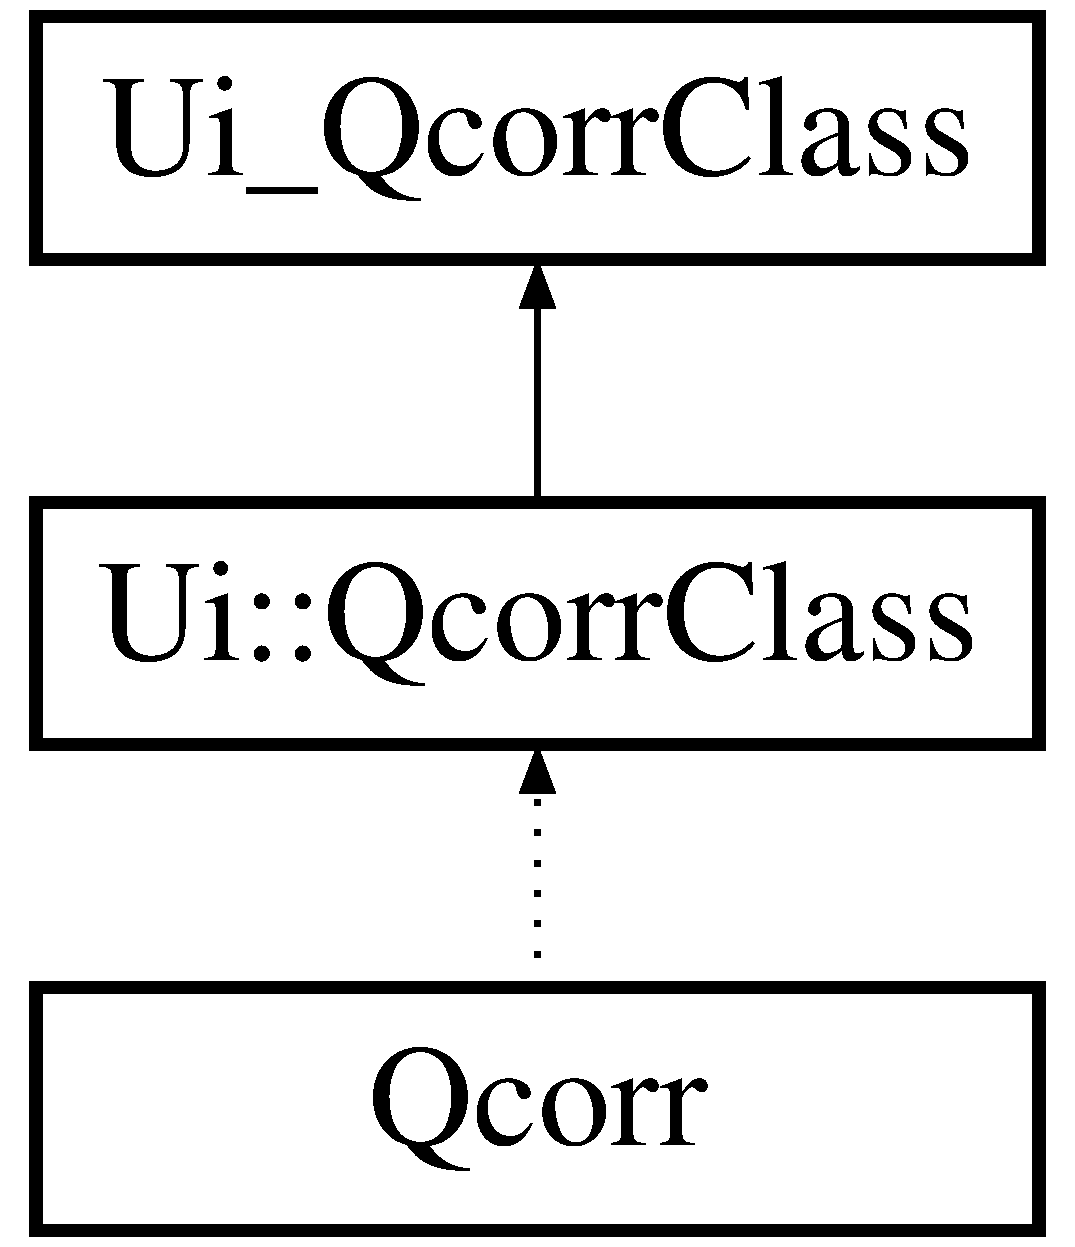
\includegraphics[height=3cm]{classUi_1_1QcorrClass}
\end{center}
\end{figure}


\subsection{Detailed Description}


Definition at line 260 of file ui\_\-qcorr.h.

The documentation for this class was generated from the following file:\begin{DoxyCompactItemize}
\item 
ui\_\-qcorr.h\end{DoxyCompactItemize}

\hypertarget{classTargetImgLabel}{
\section{TargetImgLabel Class Reference}
\label{classTargetImgLabel}\index{TargetImgLabel@{TargetImgLabel}}
}


A sub-\/classed label widget implemented with the purpose of displaying the target image on the right panel.  


{\ttfamily \#include $<$src/targetImgLabel.h$>$}\subsection*{Public Member Functions}
\begin{DoxyCompactItemize}
\item 
\hypertarget{classTargetImgLabel_acb3dcfa8b9616be0a355c90db81aaba2}{
\hyperlink{classTargetImgLabel_acb3dcfa8b9616be0a355c90db81aaba2}{TargetImgLabel} (QWidget $\ast$parent=0)}
\label{classTargetImgLabel_acb3dcfa8b9616be0a355c90db81aaba2}

\begin{DoxyCompactList}\small\item\em Constructor for the \hyperlink{classTargetImgLabel}{TargetImgLabel} class. \item\end{DoxyCompactList}\item 
void \hyperlink{classTargetImgLabel_a2ec40d8850e3d9cc4d5c9984412c0cfb}{setImage} (const QImage \&labelImage)
\begin{DoxyCompactList}\small\item\em Sets background image on this \hyperlink{classTargetImgLabel}{TargetImgLabel} class. \item\end{DoxyCompactList}\item 
void \hyperlink{classTargetImgLabel_a09dbad77c225942d7a604e06a119f60d}{overlayImage} (const QImage \&otherImage, int nXoffset=0, int nYoffset=0)
\begin{DoxyCompactList}\small\item\em Overlays an Image ontop of the current one. \item\end{DoxyCompactList}\item 
void \hyperlink{classTargetImgLabel_ab835774d14df1e93cb0fd010d1a2e699}{drawEnclosedMatch} (const QPoint originPoint, const QSize rectSize)
\begin{DoxyCompactList}\small\item\em Draws a dashed, green rectangle to indicate the position of a matching template on the target image. \item\end{DoxyCompactList}\item 
\hypertarget{classTargetImgLabel_ad060485d97c7797339243b23f3ea05ef}{
void \hyperlink{classTargetImgLabel_ad060485d97c7797339243b23f3ea05ef}{eraseEnclosedMatch} ()}
\label{classTargetImgLabel_ad060485d97c7797339243b23f3ea05ef}

\begin{DoxyCompactList}\small\item\em Erases the green rectangle that indicated a matching template on the target image. \item\end{DoxyCompactList}\end{DoxyCompactItemize}
\subsection*{Protected Member Functions}
\begin{DoxyCompactItemize}
\item 
\hypertarget{classTargetImgLabel_a30f9fc1657bdf5a9459bd78d5a94c65b}{
void \hyperlink{classTargetImgLabel_a30f9fc1657bdf5a9459bd78d5a94c65b}{paintEvent} (QPaintEvent $\ast$)}
\label{classTargetImgLabel_a30f9fc1657bdf5a9459bd78d5a94c65b}

\begin{DoxyCompactList}\small\item\em Handles the paint events by refreshing/updating the contents of this \hyperlink{classTargetImgLabel}{TargetImgLabel} class. \item\end{DoxyCompactList}\end{DoxyCompactItemize}
\subsection*{Private Attributes}
\begin{DoxyCompactItemize}
\item 
\hypertarget{classTargetImgLabel_ae532d541556a3647cff5a83bcf1306c3}{
QImage $\ast$ \hyperlink{classTargetImgLabel_ae532d541556a3647cff5a83bcf1306c3}{m\_\-image}}
\label{classTargetImgLabel_ae532d541556a3647cff5a83bcf1306c3}

\begin{DoxyCompactList}\small\item\em the right image (a.k.a target image) \item\end{DoxyCompactList}\item 
\hypertarget{classTargetImgLabel_a94cf2b5841057d54bf3172aa2fef1e83}{
QImage $\ast$ \hyperlink{classTargetImgLabel_a94cf2b5841057d54bf3172aa2fef1e83}{m\_\-overlayImage}}
\label{classTargetImgLabel_a94cf2b5841057d54bf3172aa2fef1e83}

\begin{DoxyCompactList}\small\item\em the overlaid correlation map image \item\end{DoxyCompactList}\item 
\hypertarget{classTargetImgLabel_a0ed69ba29f03494cdd3ec22d9df4e15f}{
QPoint \hyperlink{classTargetImgLabel_a0ed69ba29f03494cdd3ec22d9df4e15f}{m\_\-originPoint}}
\label{classTargetImgLabel_a0ed69ba29f03494cdd3ec22d9df4e15f}

\begin{DoxyCompactList}\small\item\em the point that indicates the top-\/left coordinates of the matching rectangle \item\end{DoxyCompactList}\item 
\hypertarget{classTargetImgLabel_ae9e4109bdd7a8a6b5d0bd59850c6abba}{
QSize \hyperlink{classTargetImgLabel_ae9e4109bdd7a8a6b5d0bd59850c6abba}{m\_\-rectSize}}
\label{classTargetImgLabel_ae9e4109bdd7a8a6b5d0bd59850c6abba}

\begin{DoxyCompactList}\small\item\em the size of the enclosing match rectangle \item\end{DoxyCompactList}\item 
\hypertarget{classTargetImgLabel_a303d7686a3dd92560851dabe82425d89}{
int \hyperlink{classTargetImgLabel_a303d7686a3dd92560851dabe82425d89}{m\_\-nXoffset}}
\label{classTargetImgLabel_a303d7686a3dd92560851dabe82425d89}

\begin{DoxyCompactList}\small\item\em X offset for overlay image. \item\end{DoxyCompactList}\item 
\hypertarget{classTargetImgLabel_a46624a74854a56d43895ecea4b2a3da5}{
int \hyperlink{classTargetImgLabel_a46624a74854a56d43895ecea4b2a3da5}{m\_\-nYoffset}}
\label{classTargetImgLabel_a46624a74854a56d43895ecea4b2a3da5}

\begin{DoxyCompactList}\small\item\em Y offset for overlay image. \item\end{DoxyCompactList}\item 
\hypertarget{classTargetImgLabel_a34a2b6061eb38412b7f7e88fbf741c2f}{
bool \hyperlink{classTargetImgLabel_a34a2b6061eb38412b7f7e88fbf741c2f}{m\_\-bHasCorrResults}}
\label{classTargetImgLabel_a34a2b6061eb38412b7f7e88fbf741c2f}

\begin{DoxyCompactList}\small\item\em indicates whether correlation results exist so an overlaid image can be composed on top of the target image \item\end{DoxyCompactList}\item 
\hypertarget{classTargetImgLabel_a3b0b34d9c2f7c4f6c9aea8bc75d91d99}{
bool \hyperlink{classTargetImgLabel_a3b0b34d9c2f7c4f6c9aea8bc75d91d99}{m\_\-bHasImage}}
\label{classTargetImgLabel_a3b0b34d9c2f7c4f6c9aea8bc75d91d99}

\begin{DoxyCompactList}\small\item\em indicates whether this \hyperlink{classTargetImgLabel}{TargetImgLabel} class has a target (main) image \item\end{DoxyCompactList}\item 
\hypertarget{classTargetImgLabel_a1c34173d16f00af22f7db9e1bb3e7b30}{
bool \hyperlink{classTargetImgLabel_a1c34173d16f00af22f7db9e1bb3e7b30}{m\_\-bHasOverlayImage}}
\label{classTargetImgLabel_a1c34173d16f00af22f7db9e1bb3e7b30}

\begin{DoxyCompactList}\small\item\em indicates whether this \hyperlink{classTargetImgLabel}{TargetImgLabel} class has an overlaid image (Usually, a correlation results map) \item\end{DoxyCompactList}\end{DoxyCompactItemize}


\subsection{Detailed Description}
A sub-\/classed label widget implemented with the purpose of displaying the target image on the right panel. A sub-\/classed label widget implemented with the purpose of displaying the target image in the right panel with added functionality such as the enclosing match visualization and overlaid correlation map images 

Definition at line 22 of file targetImgLabel.h.

\subsection{Member Function Documentation}
\hypertarget{classTargetImgLabel_ab835774d14df1e93cb0fd010d1a2e699}{
\index{TargetImgLabel@{TargetImgLabel}!drawEnclosedMatch@{drawEnclosedMatch}}
\index{drawEnclosedMatch@{drawEnclosedMatch}!TargetImgLabel@{TargetImgLabel}}
\subsubsection[{drawEnclosedMatch}]{\setlength{\rightskip}{0pt plus 5cm}void TargetImgLabel::drawEnclosedMatch (const QPoint {\em originPoint}, \/  const QSize {\em rectSize})}}
\label{classTargetImgLabel_ab835774d14df1e93cb0fd010d1a2e699}


Draws a dashed, green rectangle to indicate the position of a matching template on the target image. 
\begin{DoxyParams}{Parameters}
\item[{\em originPoint}]A QPoint that indicates the top-\/left coordinates of the matching rectangle \item[{\em rectSize}]A QSize for the matching rectangle to be drawn \end{DoxyParams}


Definition at line 107 of file targetImgLabel.cpp.

References m\_\-bHasCorrResults, m\_\-originPoint, and m\_\-rectSize.\hypertarget{classTargetImgLabel_a09dbad77c225942d7a604e06a119f60d}{
\index{TargetImgLabel@{TargetImgLabel}!overlayImage@{overlayImage}}
\index{overlayImage@{overlayImage}!TargetImgLabel@{TargetImgLabel}}
\subsubsection[{overlayImage}]{\setlength{\rightskip}{0pt plus 5cm}void TargetImgLabel::overlayImage (const QImage \& {\em otherImage}, \/  int {\em nXoffset} = {\ttfamily 0}, \/  int {\em nYoffset} = {\ttfamily 0})}}
\label{classTargetImgLabel_a09dbad77c225942d7a604e06a119f60d}


Overlays an Image ontop of the current one. 
\begin{DoxyParams}{Parameters}
\item[{\em otherImage}]Pointer to a QImage instance that will overlay the current one using Qt::CompositionMode\_\-Screen mode \item[{\em nXoffset}]X offset for overlay image. Default is 0 \item[{\em nYoffset}]Y offset for overlay image. Default is 0 \end{DoxyParams}


Definition at line 37 of file targetImgLabel.cpp.

References m\_\-bHasOverlayImage, m\_\-nXoffset, m\_\-nYoffset, and m\_\-overlayImage.\hypertarget{classTargetImgLabel_a2ec40d8850e3d9cc4d5c9984412c0cfb}{
\index{TargetImgLabel@{TargetImgLabel}!setImage@{setImage}}
\index{setImage@{setImage}!TargetImgLabel@{TargetImgLabel}}
\subsubsection[{setImage}]{\setlength{\rightskip}{0pt plus 5cm}void TargetImgLabel::setImage (const QImage \& {\em labelImage})}}
\label{classTargetImgLabel_a2ec40d8850e3d9cc4d5c9984412c0cfb}


Sets background image on this \hyperlink{classTargetImgLabel}{TargetImgLabel} class. 
\begin{DoxyParams}{Parameters}
\item[{\em labelImage}]Pointer to a QImage instance that will be used as the label's background \end{DoxyParams}


Definition at line 25 of file targetImgLabel.cpp.

References m\_\-bHasImage, m\_\-bHasOverlayImage, and m\_\-image.

The documentation for this class was generated from the following files:\begin{DoxyCompactItemize}
\item 
src/targetImgLabel.h\item 
src/targetImgLabel.cpp\end{DoxyCompactItemize}

\include{classUi__ControlsWindowClass}
\hypertarget{classUi__CorrMethodClass}{
\section{Ui\_\-CorrMethodClass Class Reference}
\label{classUi__CorrMethodClass}\index{Ui\_\-CorrMethodClass@{Ui\_\-CorrMethodClass}}
}
Inheritance diagram for Ui\_\-CorrMethodClass::\begin{figure}[H]
\begin{center}
\leavevmode
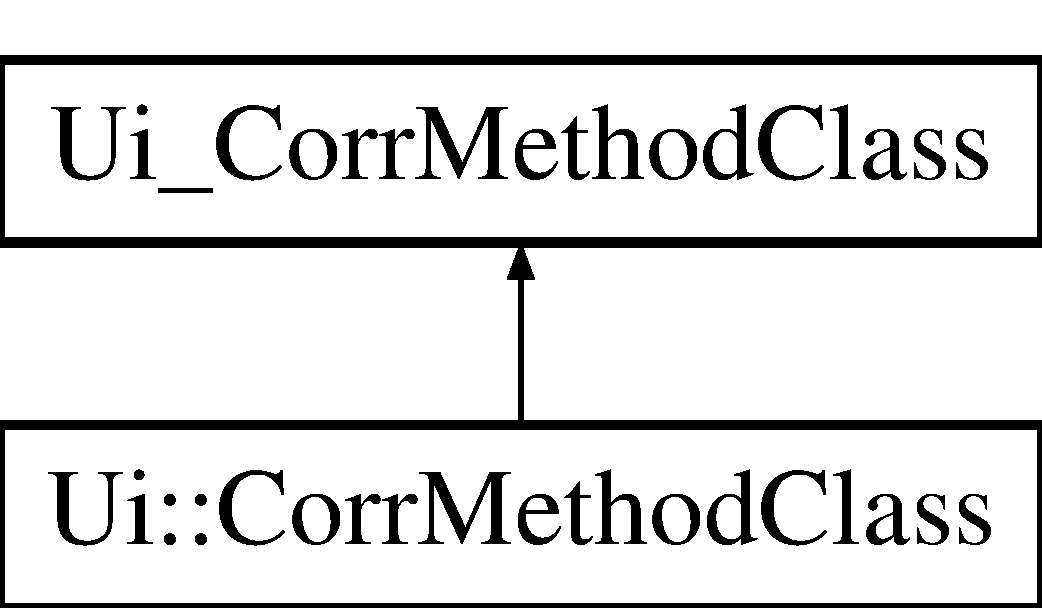
\includegraphics[height=2cm]{classUi__CorrMethodClass}
\end{center}
\end{figure}
\subsection*{Public Member Functions}
\begin{DoxyCompactItemize}
\item 
\hypertarget{classUi__CorrMethodClass_a95a6bbb76de087aa2f8f5ea4780a4d09}{
void {\bfseries setupUi} (QDialog $\ast$CorrMethodClass)}
\label{classUi__CorrMethodClass_a95a6bbb76de087aa2f8f5ea4780a4d09}

\item 
\hypertarget{classUi__CorrMethodClass_a4ac1c93be0509c13a248873b5dd7e2fb}{
void {\bfseries retranslateUi} (QDialog $\ast$CorrMethodClass)}
\label{classUi__CorrMethodClass_a4ac1c93be0509c13a248873b5dd7e2fb}

\end{DoxyCompactItemize}
\subsection*{Public Attributes}
\begin{DoxyCompactItemize}
\item 
\hypertarget{classUi__CorrMethodClass_ab3e404afe1c6fafb99e02a2a9315e8d1}{
QFrame $\ast$ {\bfseries dialog\_\-Frame}}
\label{classUi__CorrMethodClass_ab3e404afe1c6fafb99e02a2a9315e8d1}

\item 
\hypertarget{classUi__CorrMethodClass_aab4f631b545d0545adde08190ecab6fa}{
QVBoxLayout $\ast$ {\bfseries verticalLayout}}
\label{classUi__CorrMethodClass_aab4f631b545d0545adde08190ecab6fa}

\item 
\hypertarget{classUi__CorrMethodClass_add008cc6d16e9265345255c6fbc2e0b5}{
QLabel $\ast$ {\bfseries selectMethod\_\-label}}
\label{classUi__CorrMethodClass_add008cc6d16e9265345255c6fbc2e0b5}

\item 
\hypertarget{classUi__CorrMethodClass_a55e61e05e9ff340d17b08f7489e84039}{
QGroupBox $\ast$ {\bfseries methods\_\-groupBox}}
\label{classUi__CorrMethodClass_a55e61e05e9ff340d17b08f7489e84039}

\item 
\hypertarget{classUi__CorrMethodClass_aa260d1145f60cdc7137a93d50f66b2e9}{
QRadioButton $\ast$ {\bfseries method3\_\-radioButton}}
\label{classUi__CorrMethodClass_aa260d1145f60cdc7137a93d50f66b2e9}

\item 
\hypertarget{classUi__CorrMethodClass_acced16b55f7c8baa3c789435616c35c6}{
QRadioButton $\ast$ {\bfseries method2\_\-radioButton}}
\label{classUi__CorrMethodClass_acced16b55f7c8baa3c789435616c35c6}

\item 
\hypertarget{classUi__CorrMethodClass_a091300f07ee518675317d2001e486a42}{
QRadioButton $\ast$ {\bfseries method1\_\-radioButton}}
\label{classUi__CorrMethodClass_a091300f07ee518675317d2001e486a42}

\item 
\hypertarget{classUi__CorrMethodClass_ac4d190aefc50d332cfdc73d7370f4ca2}{
QDialogButtonBox $\ast$ {\bfseries buttonBox}}
\label{classUi__CorrMethodClass_ac4d190aefc50d332cfdc73d7370f4ca2}

\item 
\hypertarget{classUi__CorrMethodClass_ac98460426d7a9f1c1a2763d9e3c0c2ef}{
QSpacerItem $\ast$ {\bfseries verticalSpacer}}
\label{classUi__CorrMethodClass_ac98460426d7a9f1c1a2763d9e3c0c2ef}

\end{DoxyCompactItemize}


\subsection{Detailed Description}


Definition at line 29 of file ui\_\-corrmethod.h.

The documentation for this class was generated from the following file:\begin{DoxyCompactItemize}
\item 
ui\_\-corrmethod.h\end{DoxyCompactItemize}

\hypertarget{classUi__QcorrClass}{
\section{Ui\_\-QcorrClass Class Reference}
\label{classUi__QcorrClass}\index{Ui\_\-QcorrClass@{Ui\_\-QcorrClass}}
}
Inheritance diagram for Ui\_\-QcorrClass::\begin{figure}[H]
\begin{center}
\leavevmode
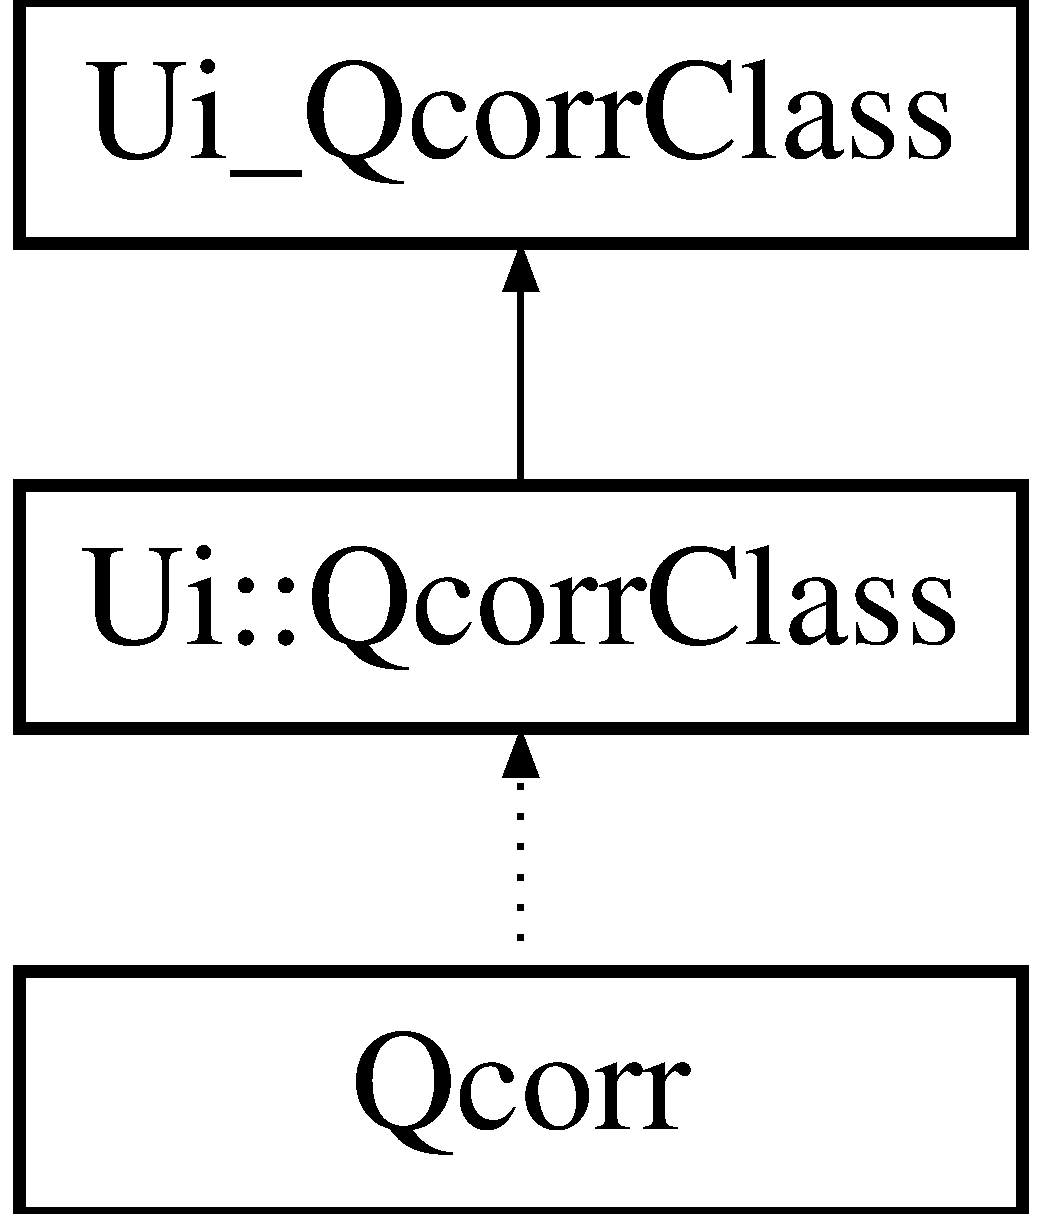
\includegraphics[height=3cm]{classUi__QcorrClass}
\end{center}
\end{figure}
\subsection*{Public Member Functions}
\begin{DoxyCompactItemize}
\item 
\hypertarget{classUi__QcorrClass_a80aee2ed06f3c4f9b1f516405d888c13}{
void {\bfseries setupUi} (QMainWindow $\ast$QcorrClass)}
\label{classUi__QcorrClass_a80aee2ed06f3c4f9b1f516405d888c13}

\item 
\hypertarget{classUi__QcorrClass_adefed69462e2297254f0d5bce3131e05}{
void {\bfseries retranslateUi} (QMainWindow $\ast$QcorrClass)}
\label{classUi__QcorrClass_adefed69462e2297254f0d5bce3131e05}

\end{DoxyCompactItemize}
\subsection*{Public Attributes}
\begin{DoxyCompactItemize}
\item 
\hypertarget{classUi__QcorrClass_ae725a71d3bb44a43e2d65ce4d1284b85}{
QAction $\ast$ {\bfseries action\_\-Quit}}
\label{classUi__QcorrClass_ae725a71d3bb44a43e2d65ce4d1284b85}

\item 
\hypertarget{classUi__QcorrClass_ae8508d05f75fac71c1f6fdb50fae6d7d}{
QAction $\ast$ {\bfseries action\_\-Correlation\_\-Map}}
\label{classUi__QcorrClass_ae8508d05f75fac71c1f6fdb50fae6d7d}

\item 
\hypertarget{classUi__QcorrClass_a885bdbbc4267078f102878ad126b23bb}{
QWidget $\ast$ {\bfseries centralwidget}}
\label{classUi__QcorrClass_a885bdbbc4267078f102878ad126b23bb}

\item 
\hypertarget{classUi__QcorrClass_acb93f5008511c2654ac8a51c17dc11ef}{
QFrame $\ast$ {\bfseries main\_\-frame}}
\label{classUi__QcorrClass_acb93f5008511c2654ac8a51c17dc11ef}

\item 
\hypertarget{classUi__QcorrClass_afd1d2aad88a740a9f33d9f91370c7ea9}{
QVBoxLayout $\ast$ {\bfseries main\_\-verticalLayout}}
\label{classUi__QcorrClass_afd1d2aad88a740a9f33d9f91370c7ea9}

\item 
\hypertarget{classUi__QcorrClass_ab4e96571e7dd58d9ec798cf6ede3cbe6}{
QSplitter $\ast$ {\bfseries splitter}}
\label{classUi__QcorrClass_ab4e96571e7dd58d9ec798cf6ede3cbe6}

\item 
\hypertarget{classUi__QcorrClass_a81e59812852e521cced5e1f912bffb99}{
QWidget $\ast$ {\bfseries layoutWidget}}
\label{classUi__QcorrClass_a81e59812852e521cced5e1f912bffb99}

\item 
\hypertarget{classUi__QcorrClass_ae7eb5196b5e392a40fa3e3a77f40c3cc}{
QVBoxLayout $\ast$ {\bfseries left\_\-verticalLayout}}
\label{classUi__QcorrClass_ae7eb5196b5e392a40fa3e3a77f40c3cc}

\item 
\hypertarget{classUi__QcorrClass_aaad53db0cbf018c38d75aebbe78959b3}{
QHBoxLayout $\ast$ {\bfseries leftImg\_\-horizontalLayout}}
\label{classUi__QcorrClass_aaad53db0cbf018c38d75aebbe78959b3}

\item 
\hypertarget{classUi__QcorrClass_a12d1c71e330c76e65484418502338a31}{
QLineEdit $\ast$ {\bfseries leftImage\_\-lineEdit}}
\label{classUi__QcorrClass_a12d1c71e330c76e65484418502338a31}

\item 
\hypertarget{classUi__QcorrClass_ae05243dcb19bfd6fd6d1c3257f25338a}{
QPushButton $\ast$ {\bfseries leftBrowse\_\-pushButton}}
\label{classUi__QcorrClass_ae05243dcb19bfd6fd6d1c3257f25338a}

\item 
\hypertarget{classUi__QcorrClass_acb12117880660e7d8fec35de7eee51c6}{
QScrollArea $\ast$ {\bfseries leftImage\_\-scrollArea}}
\label{classUi__QcorrClass_acb12117880660e7d8fec35de7eee51c6}

\item 
\hypertarget{classUi__QcorrClass_aab5ae2e7dc3baefb6ada5e1a758e826f}{
QWidget $\ast$ {\bfseries scrollAreaWidgetContents\_\-3}}
\label{classUi__QcorrClass_aab5ae2e7dc3baefb6ada5e1a758e826f}

\item 
\hypertarget{classUi__QcorrClass_a24caba38fd151a2ab5b577b1425bd07c}{
QWidget $\ast$ {\bfseries layoutWidget1}}
\label{classUi__QcorrClass_a24caba38fd151a2ab5b577b1425bd07c}

\item 
\hypertarget{classUi__QcorrClass_a232c26905d00f6608b8ba97a6546daa0}{
QVBoxLayout $\ast$ {\bfseries right\_\-verticalLayout}}
\label{classUi__QcorrClass_a232c26905d00f6608b8ba97a6546daa0}

\item 
\hypertarget{classUi__QcorrClass_a6885fe1dcc883e2f927c2fb943b206e0}{
QHBoxLayout $\ast$ {\bfseries rightImg\_\-horizontalLayout}}
\label{classUi__QcorrClass_a6885fe1dcc883e2f927c2fb943b206e0}

\item 
\hypertarget{classUi__QcorrClass_a690e51bd7f4916ca89f876f39afee05d}{
QLineEdit $\ast$ {\bfseries rightImage\_\-lineEdit}}
\label{classUi__QcorrClass_a690e51bd7f4916ca89f876f39afee05d}

\item 
\hypertarget{classUi__QcorrClass_a5018f953d94c196394a638212a45fd9d}{
QPushButton $\ast$ {\bfseries rightBrowse\_\-pushButton}}
\label{classUi__QcorrClass_a5018f953d94c196394a638212a45fd9d}

\item 
\hypertarget{classUi__QcorrClass_a227cae34e275c9e0713ee279435f41cc}{
QScrollArea $\ast$ {\bfseries rightImage\_\-scrollArea}}
\label{classUi__QcorrClass_a227cae34e275c9e0713ee279435f41cc}

\item 
\hypertarget{classUi__QcorrClass_abf4b50d1ea6274629f687ac66ce12e80}{
QWidget $\ast$ {\bfseries scrollAreaWidgetContents\_\-2}}
\label{classUi__QcorrClass_abf4b50d1ea6274629f687ac66ce12e80}

\item 
\hypertarget{classUi__QcorrClass_aa4247652a1ed71c6b6704aa3273544bd}{
QHBoxLayout $\ast$ {\bfseries bottom\_\-horizontalLayout}}
\label{classUi__QcorrClass_aa4247652a1ed71c6b6704aa3273544bd}

\item 
\hypertarget{classUi__QcorrClass_a06bd40ad7db57a5438d16e5d5061df42}{
QPushButton $\ast$ {\bfseries corr\_\-pushButton}}
\label{classUi__QcorrClass_a06bd40ad7db57a5438d16e5d5061df42}

\item 
\hypertarget{classUi__QcorrClass_a4ddf4aae819f6b25476a5a3e76c600d7}{
QLabel $\ast$ {\bfseries corrResults\_\-label}}
\label{classUi__QcorrClass_a4ddf4aae819f6b25476a5a3e76c600d7}

\item 
\hypertarget{classUi__QcorrClass_a80762eea1a44f16ceffed065d0459a69}{
QSpacerItem $\ast$ {\bfseries horizontalSpacer}}
\label{classUi__QcorrClass_a80762eea1a44f16ceffed065d0459a69}

\item 
\hypertarget{classUi__QcorrClass_ad032c2f5b8f1aed8decad689900d7017}{
QPushButton $\ast$ {\bfseries quit\_\-pushButton}}
\label{classUi__QcorrClass_ad032c2f5b8f1aed8decad689900d7017}

\item 
\hypertarget{classUi__QcorrClass_a8567acdc882322bab775dd04569433da}{
QMenuBar $\ast$ {\bfseries menubar}}
\label{classUi__QcorrClass_a8567acdc882322bab775dd04569433da}

\item 
\hypertarget{classUi__QcorrClass_a1d52a371f0d1e29cdf70d1be2a85a45e}{
QMenu $\ast$ {\bfseries menu\_\-Menu}}
\label{classUi__QcorrClass_a1d52a371f0d1e29cdf70d1be2a85a45e}

\item 
\hypertarget{classUi__QcorrClass_a8c1dd90b9ea2130b6fe6e8e6553fbf13}{
QMenu $\ast$ {\bfseries menu\_\-View}}
\label{classUi__QcorrClass_a8c1dd90b9ea2130b6fe6e8e6553fbf13}

\item 
\hypertarget{classUi__QcorrClass_ae220680c312c600f015f0413ad6cd2cf}{
QStatusBar $\ast$ {\bfseries statusbar}}
\label{classUi__QcorrClass_ae220680c312c600f015f0413ad6cd2cf}

\end{DoxyCompactItemize}


\subsection{Detailed Description}


Definition at line 35 of file ui\_\-qcorr.h.

The documentation for this class was generated from the following file:\begin{DoxyCompactItemize}
\item 
ui\_\-qcorr.h\end{DoxyCompactItemize}

\printindex
\end{document}
